\documentclass[11pt, letterpaper]{article}

% Encoding
\usepackage[T1]{fontenc} % Output
\usepackage[latin1]{inputenc} % Input

% MATHS
\usepackage{amsmath, amssymb, amsfonts} % Math stuff

% linenofix -------------------------------------------
\newcommand*\patchAmsMathEnvironmentForLineno[1]{%
  \expandafter\let\csname old#1\expandafter\endcsname\csname #1\endcsname
  \expandafter\let\csname oldend#1\expandafter\endcsname\csname end#1\endcsname
  \renewenvironment{#1}%
     {\linenomath\csname old#1\endcsname}%
     {\csname oldend#1\endcsname\endlinenomath}}% 
\newcommand*\patchBothAmsMathEnvironmentsForLineno[1]{%
  \patchAmsMathEnvironmentForLineno{#1}%
  \patchAmsMathEnvironmentForLineno{#1*}}%
\AtBeginDocument{%
\patchBothAmsMathEnvironmentsForLineno{equation}%
\patchBothAmsMathEnvironmentsForLineno{align}%
\patchBothAmsMathEnvironmentsForLineno{flalign}%
\patchBothAmsMathEnvironmentsForLineno{alignat}%
\patchBothAmsMathEnvironmentsForLineno{gather}%
\patchBothAmsMathEnvironmentsForLineno{multline}%
}
%-----------------------------------------------------

\usepackage{mhsetup, mathtools, empheq} % Other optional maths stuff
\usepackage{mathrsfs}
\usepackage{amsthm}
\newenvironment{myproof}{\begin{proof}[\unskip\nopunct]}{\end{proof}}

% FORMATTING
\usepackage{array} % Tables etc
\usepackage{longtable} % Break table over pages
\usepackage{pdflscape} % to turn table in landscape mode

\usepackage{multirow} % Join cells over multiple rows
\usepackage{paralist} % In-paragraph itemized lists (\begin{inparaenum}\item.... \end{inparaenum})
\usepackage{lineno} % For line numbering
\usepackage{setspace} % Line spacing
\usepackage{nameref} % Reference to section name, not just number

\usepackage{chngcntr} % For equation counter in the appendix

% Date format
\usepackage[iso, english]{isodate}


% HEAD AND FOOT
\usepackage{lastpage}
\usepackage{fancyhdr}
\fancypagestyle{maintext}{
\fancyhf{}
\fancyhead[C]{}
\fancyfoot[C]{\thepage/\pageref{LastPage}}
\fancyfoot[R]{\footnotesize \today}
\renewcommand{\headrulewidth}{0.pt}
}

\fancypagestyle{appendix}{
\fancyhf{}
\fancyhead[C]{{Appendix \thesection{}}}
\fancyfoot[C]{\thepage/\pageref{LastPage}}
\renewcommand{\headrulewidth}{0.02pt}
\fancyfoot[R]{\today}
}

% BIBLIOGRAPHY
\usepackage[]{natbib} % Package for the bibliography

% Colors
\usepackage[table]{xcolor}
\definecolor{dgray}{gray}{0.3}
\definecolor{seccol}{HTML}{4080BF}
\definecolor{subseccol}{HTML}{336699}
\definecolor{subsubseccol}{HTML}{264d73}
\definecolor{parcol}{HTML}{19334d}
% TABLES
\usepackage{tabu}


% FIGURES
% Package to label the different panels of a figure
\usepackage[FIGTOPCAP, raggedright, sf, bf, scriptsize, SF, nooneline]{subfigure} 
% Tikz and related packages (to draw figures)
\usepackage{tikz}
\usetikzlibrary{positioning, arrows,trees, shapes, fit, calc}
% Style of the captions
\usepackage[font={small,sf, doublespacing}, labelfont=bf]{caption}


\usepackage{floatrow}

%% FONTS
% Fonts of the main text
\usepackage{fourier}
% Helvetica for sans serif fonts
\renewcommand{\sfdefault}{phv}
% Make sure mathcal looks the same
\DeclareMathAlphabet{\mathcal}{OMS}{cmsy}{m}{n}

% SECTIONS
\usepackage{titlesec}
\usepackage{needspace}

%% Section
\titleformat{\section}[block]
  {\needspace{2in}\Large \bfseries \color{seccol}}
  {\thesection}
  {1em}
  {}
% Subsection
\titleformat{\subsection}[block]
  {\large\bfseries \color{subseccol}}
  {\thesubsection}
  {1em}
  {} 
% Subsubsection
\titleformat{\subsubsection}[block]
  {\bfseries \color{subsubseccol}}
  {\thesubsubsection}
  {1em}
  {} 
% Paragraph
\titleformat{\paragraph}[runin]
  {\normalsize\bfseries \color{parcol}}
  {\theparagraph}
  {0em}
  {}

% TABLES
\usepackage{multirow}
\usepackage{rotating}

\usepackage[colorlinks=true, citecolor=black, linkcolor=black, urlcolor=black]{hyperref}
\hypersetup{
%    pdftitle={Mutation and social evolution},
 %   pdfauthor={Your name here},
 %   pdfsubject={Your subject here},
  %  pdfkeywords={keyword1, keyword2},
  %  bookmarksnumbered=true,     
    bookmarksopen=true,         
  %  bookmarksopenlevel=1,       
  %  colorlinks=true,            
    pdfstartview=Fit,           
    pdfpagemode=UseOutlines,    % this is the option you were lookin for
  %  pdfpagelayout=TwoPageRight
}


% STYLES IMPORTED FOR EQREF DOCUMENT
\makeatletter 
\renewcommand{\eqref}[1]{\textup{{\normalfont eq.~(\ref{#1}}\normalfont)}}
\makeatother
\newcommand{\Eqref}[1]{Eq.~(\ref{#1})}
\newcommand{\sysref}[1]{system~(\ref{#1})}
\newcommand{\Sysref}[2]{System~(\ref{#1})}

\usepackage{mathrsfs}
\usepackage{dsfont} % Mathbb for 1


%%% STUFF TO COMMENT OUT FOR THE FINAL VERSION 
\usepackage{soul} % Highlighting (command \hl{})
\usepackage{todonotes} % Add Word-style comments (\todo{})
\usepackage[final]{showlabels} % To display the labels of the equations on the pdf; 
\usepackage[top = 1.15in, bottom = 1.25in, left = 1.75in, right = 1.75in]{geometry}
%\geometry{textwidth=0.65\paperwidth}
%%%

\newcommand{\ie}{\textit{i.e.}}
\newcommand{\eg}{\textit{e.g.}}
\newcommand{\vs}{\textit{vs.\ }}

\newcommand{\deriv}[2]{\partial_{#2}\!{#1}\,}
%\newcommand{\deriv}[2]{\left.\frac{\partial #1}{\partial #2}\right |_{#2=0}}
\newcommand{\derivv}[3]{\left.\frac{\partial #1}{\partial #2}\right |_{#3=0}} % Version of \deriv with different evaluation
\newcommand{\derivvv}[3]{\left.\frac{\partial #1}{\partial #2}\right |_{#3}} % Version of \deriv with different evaluation
\newcommand{\sderivv}[3]{\partial_{#2}\!{#1}\,} % Version of \deriv with different evaluation, shorter

% Expectations and Probabilities
\newcommand{\Esp}[1]{\mathbb{E}\big[ #1\big]}%{\mathbb{E}\left[ #1\right]}
\newcommand{\Espzero}[1]{\mathbb{E}_0\big[ #1\big]}%{\mathbb{E}\left[ #1\right]}
\newcommand{\Espt}[2]{\mathbb{E}_{#2}\big[ #1\big]}%{\mathbb{E}\left[ #1\right]}
\newcommand{\Prob}[1]{\mathbb{P}\left[ #1\right]}
\newcommand{\Probzero}[1]{\mathbb{P}_0\left[ #1\right]}
 
\newcommand{\bigO}[1]{O\left( #1 \right)}
\newcommand{\Tr}[1]{\textrm{Tr}\left( #1\right)}

\newcommand{\subst}[1]{\scriptsize \substack{ #1}}
\newcommand{\justif}[1]{\quad \textrm{\small [#1]}}

\newcommand{\ssum}[2]{{\textstyle \sum\limits_{#1}^{#2}}}

\newcommand{\appname}[0]{Appendix}

% NOTATION FOR QUELLER TYPE MATRIX
\newcommand{\bb}{\mathsf{b}}
\newcommand{\cc}{\mathsf{c}}
\newcommand{\dd}{\mathsf{d}}

\newcommand{\direct}{\mathrm{D}}
\newcommand{\indirect}{\mathrm{I}}

\newcommand{\makemat}[1]{\mathbf{#1}}
\newcommand{\Pin}{P_{\textrm{in}}}
\newcommand{\Pout}{P_{\textrm{out}}}

\newcommand{\Moran}{\textrm{M}}
\newcommand{\BD}{\textrm{BD}}
\newcommand{\DB}{\textrm{DB}}
\newcommand{\WF}{\textrm{WF}}

\newcommand{\mutbias}{\nu}
\makeatletter
\let\thetitle\@title
\let\theauthor\@author
\makeatother

\usepackage{hyphenat}

\newcommand{\self}{\textrm{self}}
\newcommand{\inn}{\textrm{in}}
\newcommand{\out}{\textrm{out}}
\newcommand{\ein}{e_{\inn}}
\newcommand{\eself}{e_{\self}}
\newcommand{\eout}{e_{\out}}
\newcommand{\din}{d_{\inn}}
\newcommand{\dself}{d_{\self}}
\newcommand{\dout}{d_{\out}}
\newcommand{\Qin}{Q_{\inn}}
\newcommand{\Qout}{Q_{\out}}

\newcommand{\ndemes}{N_D}
% FLUSH FIGURES IN THE END
%\usepackage[tablesonly]{endfloat}

\usepackage[fighead, nofiglist, nomarkers]{endfloat}
%\renewcommand{\efloatseparator}{}

\newcommand{\defeq}{\mathrel{\mathop:}=}

\newcommand{\myphantom}{\phantom{\overline{f}}}

\def \wpic {4.5cm}

\begin{document}
\pagestyle{maintext}

%TC:ignore 

\paragraph{Article Type:} Letter

\paragraph{Article Title:} Imperfect strategy transmission can reverse the role of population viscosity on the evolution of altruism .

\paragraph{Author:} Florence D\'ebarre -- Centre Interdisciplinaire de Recherche en Biologie (CIRB), Coll\`ege de France, CNRS UMR 7241 - Inserm U1050, 11 place Marcelin Berthelot, 75231 Paris Cedex 05, France. \texttt{florence.debarre@normalesup.org}

\paragraph{Short Running Title:} Mutation and altruism in subdivided populations.

\paragraph{Keywords:} Altruism, Subdivided population, Mutation, Migration, Cooperation, Island model.
%(Up to 10)

\paragraph{Word Count:}
\begin{tabular}[t]{ll}
Abstract & $172$ \\
Impact summary & $282$ words \\
Total & $4234$ words
\end{tabular}

%\paragraph{Abstract Word Count:} Should be below 300 words

%\paragraph{Total Word Count:}a\\ Authors should aim to keep the word count below 5000 words. The Abstract, Impact statement, Acknowledgements, Author Contributions and Data Accessibility sections do not contribute towards the word count.

\todo[inline]{Check $\omega$ removes entirely + explain delta in table}

\linenumbers
\subsubsection*{Abstract}
\doublespacing
Population viscosity, \ie, low emigration out of the natal deme, leads to high within-deme relatedness, which is beneficial to the evolution of altruistic behavior when social interactions take place among deme-mates. At the same time however, it increases competition among related individuals. The evolution of altruism depends on the balance between these opposite effects. This balance is already known to be affected by details of the life-cycle; we show here that it further depends on the fidelity of strategy transmission from parents to their offspring. We consider different life-cycles (Wright-Fisher, with synchronous non-overlapping generations, Moran Death-Birth and Moran Birth-Death, both with exactly one individual dying and reproducing at each time step) and we identify thresholds of parent-offspring strategy transmission inaccuracy, above which the effect of population viscosity on the frequency of altruists maintained in the population qualitatively changes. Analytical predictions are first obtained analytically under weak selection and equal deme sizes, then confirmed with stochastic simulations relaxing these assumptions. This result challenges the notion that the evolution of altruism requires limited dispersal. 

\clearpage
\subsubsection*{Impact Summary}

The evolution of altruistic behavior has fascinated and puzzled evolutionary biologists for a long time: how can a strategy whereby individuals help others at their own cost be maintained in a population? One answer is the fact that altruists may interact with other altruists more often than non-altruists do, a situation made possible by spatial structure and low emigration. Low emigration indeed means that an individual is mostly surrounded by related individuals; when social strategies are faithfully transmitted from parents to offspring, and social interactions are local as well, then altruists interact mainly with other altruists. However, this also means that related individuals have to compete against each other. Whether altruism eventually evolves depends on the balance between these beneficial and detrimental consequences of low emigration. Previous work has shown that the balance depends on the life-cycle that the population undergoes; under nearly perfect strategy transmission, low emigration goes from being neutral to the evolution of altruism (when generations are synchronous and non-overlapping) to favorable. In this work, we show that this conclusion qualitatively changes when offspring do not necessarily adopt their parent's strategy, that is, when strategy transmission is imperfect. This can be due to mutation when transmission is genetic, but also to imperfect vertical cultural transmission. We identify thresholds of strategy transmission infidelity, above which higher emigration is more conducive to the evolution of altruism than low emigration. The predictions are first obtained mathematically under the restrictive assumptions that selection is weak and that all demes have the same size, but are then confirmed with computer simulations relaxing these assumptions. This work shows that the evolution of altruism does not require -- and even can be hampered by -- low emigration. 


%Authors should provide an approximately 300 word summary, explaining why the article makes an important contribution to Evolutionary Biology. It should be accessible to a wide audience, e.g. journalists, non-expert public interested in evolution, school science teachers.



\clearpage

%TC:endignore 


\section{Introduction}%
In his pioneering work on the evolution of social behavior, \citeauthor{Hamilton1964} suggested that altruistic behavior would be associated to limited dispersal \citep[p.~10]{Hamilton1964}. This notion, that tighter links between individuals favor the evolution of altruism, has been shown to hold in a number of population structures  \citep[see \eg][]{Ohtsuki2006, TaylorDayWild2007, Lehmann2007}. The rationale that altruism is favored when altruists interact more with altruists than defectors do (\citealp[p.~141]{Hamilton1975}; \citealp{Fletcher2009})%http://www.jstor.org/stable/10.1086/338945?seq=6#page_scan_tab_contents
, a condition that is met in viscous populations, \ie, populations with limited dispersal.

Yet, living next to your kin also implies competing against them \citep{West2002}. The evolution of social traits hence depends on the balance between the positive effects of interactions with related individuals and the detrimental consequences of kin competition. Under specific conditions, the two effects can even compensate each other, thereby annihilating the impact of population viscosity on the evolution of altruism. 
First identified with computer simulations \citep{Wilson1992}, this cancellation result was analyzed by \citet{Taylor1992islandmodel} in a model with synchronous generations (\ie, Wright-Fisher model) and a subdivided population of constant, infinite size. The cancellation result was later extended to heterogeneous populations \citep[][with synchronous generations and infinite population size]{RodriguesGardner2012}, and other life-cycles, with generic regular population structures \citep[][with synchronous generations but also with continuous generations and Birth-Death updating]{Taylor2011}. However, small changes in the model's assumptions, such as overlapping generations \citep{TaylorIrwin2000} or the presence of empty sites \citep{Alizon2008} can tip the balance back in the favor of altruism. 
This high dependence on life-cycle specificities highlights the difficulty of making general statements about the role of spatial structure on the evolution of altruism. 
In this study, we will consider three different life-cycles: Wright-Fisher, where the whole population is renewed at each time step, and two Moran life-cycles (Birth-Death and Death-Birth), where a single individual dies and is replaced at each time step. 

A large number of studies on the evolution of social behavior consider simple population structures (typically, homogeneous populations \textit{sensu} \citet[][]{TaylorDayWild2007}) and often also infinite population sizes \citep[but see][for results on any structure]{Allen2017}. 
These studies also make use of weak selection approximations, and commonly assume rare \citep[\eg,][]{LeturqueRousset2002, Taylor2007JTB, TarnitaTaylor2014} or absent mutation \citep[for models assuming infinite population sizes, or models concentrating on fixation probabilities][for recent reviews]{LehmannRousset2014,VanCleve2015}. 
Often, these simplifying assumptions are a necessary step towards obtaining explicit analytical results. 
Although artificial, simple population structures (\eg, regular graphs, or subdivided populations with demes of equal sizes) help reduce the dimensionality of the system under study, in particular when the structure of the population displays symmetries such that all sites behave the same way in expectation. 
Weak selection approximations are crucial for disentangling spatial moments \citep{Lion2016}, that is, changes in global \vs local frequencies \citep[though they can in some cases be relaxed, as in][]{MullonLehmann2014}. 
Mutation, however, is usually ignored by classical models of inclusive fitness because these models assume infinite population sizes, so that there is no need to add mechanisms that restore genetic diversity \citep{TarnitaTaylor2014}. In populations of finite size,  this diversifying effect can be obtained thanks to mutation. %Mutation, and more generally imperfect strategy transmission, can alter evolutionary dynamics, in particular in spatially structured populations \citep[see \eg,][for graph-structured populations]{Allen2012,Debarre2017}. The aim of this study is hence to explore whether and how imperfect strategy transmission from parents to their offspring affects the impact of population viscosity on the evolution of altruistic behavior in subdivided populations.

When strategy transmission is purely genetic, it makes sense to assume that mutation is relatively weak. A social strategy can however also be culturally transmitted from parent to offspring, in which case ``rebellion'' (as in \citeauthor{Frank1997}'s Rebellious Child Model \citep{Frank1997}) does not have to be rare. Imperfect strategy transmission can alter evolutionary dynamics, in particular in spatially structured populations \citep[see \eg,][for graph-structured populations]{Allen2012,Debarre2017}. Here, we want to explore the consequences of imperfect strategy transmission from parents to their offspring on the evolution of altruistic behavior in subdivided populations. For the sake of concision, we use the word ``mutation'' throughout the paper, keeping in mind that strategy transmission does not have to be genetic. 

For each of the three life-cycles that we consider, we compute the expected (\ie, long-term) frequency of altruists maintained in a subdivided population, and investigate how it is affected by mutation and emigration. We find that, contrary to what happens with perfect strategy transmission, higher emigration can increase the expected frequency of altruists in the population. 
%imperfect strategy transmission from parent to offspring can qualitatively alter the way population viscosity affects the expected frequency of altruists in the population: emigration can 

% -> ABSTRACT?
%The aim of this study is to explore whether and how imperfect strategy transmission from parents to their offspring affects the impact of population viscosity on the evolution of altruistic behavior. We consider a population of fixed size, subdivided into demes of equal sizes, whose individuals reproduce asexually, and where the probability of emigrating away from the parental deme tunes the viscosity of the population. We focus on three different life-cycles (Wright-Fisher, Moran Birth-Death and Moran Death-Birth); for each of them, we compute the expected frequency of altruists in the population, and dissect the influence of direct and indirect (\ie, competitive) effects.  and determine for each of them what is the expected proportion of altruists, and we will see that non zero mutation probabilities can qualitatively alter the way population viscosity affects the expected frequency of altruists in the population. We identify thresholds of mutation probability above which the expected frequency of altruists increases with the emigration probability. 



\section{Model and methods}

\subsection{Assumptions}

We consider a population of size $N$, subdivided into $\ndemes$~demes, each hosting exactly $n$ individuals (\ie, each deme contains $n$ sites, each of which is occupied by exactly one individual; we have $n \ndemes = N$). Each site has a unique label $i$, $1\leq i \leq N$. There are two types of individuals in the population, altruists and defectors. The type of the individual living at site $i$ ($1\leq i \leq N$) is given by an indicator variable $X_i$, equal to $1$ if the individual is an altruist, and to $0$ if it is a defector. The state of the entire population is given by a $N$-long vector $\mathbf{X}$. For a given population state $\mathbf{X}$, the proportion of altruists is $\overline{X} = \sum_{i=1}^N X_i$. All symbols are summarized in table~\ref{tab:symbols}.

Reproduction is asexual. Parents transmit their strategy to their offspring with probability $1-\mu$; this transmission can be genetic or cultural (vertical cultural transmission), but for simplicity, we refer to the parameter $\mu$ as a mutation probability. With probability $\mu$, offspring do not inherit their strategy from their parent but instead get one randomly: with probability $\mutbias$, they become altruists, with probability $1-\mutbias$ they become defectors. We call the parameter $\mutbias$ the mutation bias. 

% Social interactions and effect on fecundity (simple version). 
An individual of type $X_k$ expresses a social phenotype $\phi_k = \delta X_k$, where $\delta$ is assumed to be small ($\delta \ll 1$). Social interactions take place within each deme; each individual interacts with the $n-1$ other deme members. Denoting by $e_{ij}$ the interaction probability between individuals living at sites $i$ and $j$, we have $e_{ij} = 1/(n-1)$ if $i$ and $j$ are two different sites in the same deme, and $e_{ij}=0$ otherwise. We assume that social interactions affect individual fecundity; $f_k$ denotes the fecundity of the individual at site $k$. The baseline fecundity, \ie{} individual fecundity when no altruists are present in the population, is set equal to $1$. We denote by $\bb$ the marginal effect of a deme-mate's phenotype on the fecundity of a focal individual, and by $-\cc$ the marginal effect of a focal individual's phenotype on its own fecundity ($\cc \leq \bb$). With these assumptions are notation, at the first order in $\delta$, the fecundity of the individual living at site $k$ is given by\todo{remove?} 
\begin{equation}\label{eq:deff}
f_k(\mathbf{X}, \delta) = 1 + \delta \left( \sum_{\ell =1}^N e_{\ell k} \bb X_{\ell} - \cc X_k \right) + \bigO{\delta^2}.
\end{equation}

% Dispersal - emigration
Offspring remain in the parental deme with probability $1-m$; when they do, they land on any site of the deme with equal probability (including the very site of their parent). With probability $m$, offspring emigrate to a different deme, chosen uniformly at random among the other demes. Denoting by $d_{ij}$ the probability of moving from site $i$ to site $j$, we have
\begin{equation}\label{eq:defD}
d_{ij} = \begin{cases}
 \din =  \frac{1-m}{n} & \textrm{if both sites are in the same deme;}\\
 \dout = \frac{m}{(\ndemes-1) n} & \textrm{if the two sites are in different demes,} 
\end{cases}
\end{equation}
%
with $0 < m < 1-\frac{1}{\ndemes}$ (the upper bound implies $\din>\dout$).

% Life-cycles
We denote by $B_i = B_i(\mathbf{X}, \delta)$ the expected number of successful offspring of the individual living at site $i$ (successful means alive at the next time step), and by $D_i = D_i(\mathbf{X}, \delta)$ the probability that the individual living at site $i$ dies. Both depend on the state of the population $\mathbf{X}$, but also on the way the population is updated from one time step to the next, \ie, on the chosen life-cycle (also called updating rule). We will specifically explore three different life-cycles. At the beginning of each step of each life-cycle, all individuals produce offspring, that can be mutated; then these juveniles move, within the parental deme or outside of it, and land on a site. The next events occurring during the time step depend on the life-cycle:
\begin{description}
\item[Moran Birth-Death]: One of the newly created juveniles is chosen at random; it kills the adult who was living at the site, and replaces it; all other juveniles die. 
\item[Moran Death-Birth]: One of the adults is chosen to die (uniformly at random among all adults). It is replaced by one of the juveniles who had landed in its site. All other juveniles die. 
\item[Wright-Fisher]: All the adults die. At each site of the entire population, one of the juveniles that landed there is chosen and establishes at the site. 
\end{description}
  
\subsection{Methods}
\subsubsection{Analytical part}

The calculation steps to obtain the expected (\ie, long-term) proportion of altruists are given in \appname~\ref{sec:app:EX}. They go as follows: first, we write an equation for the expected frequency of altruists in the population at time $t+1$, conditional on the composition of the population at time $t$; we then take the expectation of this quantity and consider large times $t$. After this, we write a first order expansion for phenotypic differences $\delta$ close to $0$ (this corresponds to weak selection approximation). 

The formula involves quantities that can be identified as neutral probabilities of identity by descent $Q_{ij}$, \ie, the probability that individuals living at site $i$  and $j$ share a common ancestor and that no mutation occurred on either lineage since that ancestor, in a model with no selection ($\omega=0$ -- this is the ``mutation definition'' of identity by descent \citep{RoussetBilliard2000}.)

These neutral probabilities of identity by descent depend on the chosen life-cycle, and are also computed by taking the long-term expectation of conditional expectations after one time step (see \appname~\ref{sec:app:IBD} and \ref{sec:app:Qsubdiv}). 

All the results obtained analytically were checked numerically using specific population structures (see supplementary Mathematica file \citep{Mathematica11}.)

\subsubsection{Stochastic simulations}
We also ran stochastic simulations (coded in \texttt{C}). The simulations were run for $10^8$ generations (one generation is one time step for the Wright-Fisher life-cycle, and $N$ time steps for the Moran life-cycles). For each set of parameters and life-cycle, using R \citep{R2015}, we estimated the long-term frequency of altruists by sampling the population every $10^3$ generations and computing the average frequency of altruists.\\
%
All scripts are available at \\
{\small \url{https://github.com/flodebarre/SocEvolSubdivPop/tree/master/Programs}} 

\section{Results}

\subsection{Probabilities of identity by descent}

As we will see later, the expected frequencies of altruists in the population depend on probabilities of identity by descent of pairs of sites, $Q_{ij}$. Two individuals are said to be identical by descent if there has not been any mutation on either lineage since their common ancestor.  Because of the structure of the population, there are only three types of pairs of individuals, and hence three different values of the probabilities of identity by descent of pairs of sites $Q_{ij}$:
\begin{equation}
Q_{ij} = 
\begin{cases}
1 & \textrm{when $i=j$;}\\
%
\Qin & \textrm{when $i\neq j$ and both sites are in the same deme;}\\
%
\Qout & \textrm{when sites $i$ and $j$ are in different demes.}
\end{cases}
\end{equation}
The values of $\Qin$ and $\Qout$ depend on the type of life-cycle that we consider. 

\subsubsection{Moran updating} 

Under the Moran life-cycles, probabilities of identity by descent satisfy, for any pair of sites $i$ and $j\neq i$,
\begin{equation}
Q_{ij}^{\Moran} = \frac{1-\mu}{2} \sum_{k=1}^N \left(d_{kj} Q_{ki}^{\Moran} + d_{ki} Q_{kj}^{\Moran}\right).
\end{equation}
%
Given the law of total probabilities, we first consider the site that was last updated ($1/2$ chance that it was $j$ rather than $i$); then we consider each potential parent $k$, weighted by the dispersal probabilities $d_{kj}$. Then the individuals at sites $i$ and $j$ are identical by descent (IBD) if $i$ and $j$'s parent were IBD ($Q_{ki}^{\Moran}$) and if no mutation occurred ($1-\mu$).  Replacing the dispersal probabilities $d_{ij}$ by their values (given in \eqref{eq:defD}), we eventually obtain (see \appname~\ref{sec:app:IBD} for calculation steps):
\begin{subequations}\label{eq:QM}
\begin{align}
\Qin^{\Moran} &= \frac{(1-\mu ) \left(m + \mu  (\ndemes (1-m)-1)\right)}{(1-\mu ) m (\ndemes \mu  (n-1)+1)+(\ndemes-1) \mu  (\mu  (n-1)+1)},\\
%
%
\Qout^{\Moran} & = \frac{(1-\mu ) m}{(1-\mu ) m (\ndemes \mu  (n-1)+1)+(\ndemes-1) \mu  (\mu  (n-1)+1)}.
\end{align}
\end{subequations}
%
The probability that two different deme-mates are identical by descent, $\Qin^{\Moran}$, decreases monotonically with the emigration probability $m$, while  $\Qout^{\Moran}$ monotonically increases with $m$ (see figure~\ref{fig:Q}\subref{fig:sub:QM}). 

When the mutation probability $\mu$ is vanishingly small ($\mu \to 0$), both $\Qin^{\Moran}$ and $\Qout^{\Moran}$ are equal to $1$: in the absence of mutation indeed, the population ends up fixed for one of the two types, and all individuals are identical by descent. Note that we obtain a different result if we first assumed that the size of the population is infinite ($\ndemes \to \infty$), because the order of limits matters; %  ($\lim_{d\to\infty} \lim_{\mu\to0} \Qin^{M} \neq  \lim_{\mu\to0} \lim_{d\to\infty}   \Qin^{M}$).
for instance, $\lim_{d\to \infty} \Qout^{M}=0$. 


\subsubsection{Wright-Fisher updating}

Under a Wright-Fisher life-cycle, generations are synchronous: all individuals are replaced at each time step. Probabilities of identity by descent satisfy, for any pair of sites $i$ and $j \neq i$
\begin{equation}
Q_{ij}^{\WF} = (1-\mu)^2 \sum_{k,\ell = 1}^N d_{ki} d_{\ell j} Q_{kl}^{\WF}.
\end{equation}
The sum is over all possible parents $k$ and $\ell$ of $i$ and $j$, weighted by the dispersal probabilities to sites $i$ and $j$; the individuals at sites $i$ and $j$ are identical by descent if their parents were ($Q_{k\ell}$) and if neither mutated ($(1-\mu)^2$). 

Replacing the dispersal probabilities $d_{ij}$ by their values (given in \eqref{eq:defD}) and skipping calculation steps (but see \appname~\ref{sec:app:IBD} for details), we obtain:
%
\begin{subequations}\label{eq:QWF}
\begin{align}
\Qin^{\WF} &= \frac{-\ndemes + M_1 + M_2}{(n-1) \ndemes +M_1 + M_2}, \\
\Qout^{\WF} & = \frac{-\frac{1}{\ndemes-1}M_1 + M2}{(n-1) \ndemes +M_1 + M_2},
\end{align}
with
\begin{equation*}
M_1 = \frac{\ndemes-1}{1-\frac{(1-\mu )^2 (\ndemes (1-m)-1)^2}{(\ndemes-1)^2}} \textrm{ and }M_2 = \frac{1}{1-(1-\mu)^2}.
\end{equation*}
\end{subequations}
%
(These formulas are compatible with, \eg, results presented by \citet{CockerhamWeir1987}, adapted for haploid individuals).\\
In the Wright-Fisher life-cycle, $\Qin^{\WF}$ decreases until $m=m_c^{\WF} = \frac{d-1}{d}$, then increases again, while $\Qout^{WF}$ follows the opposite pattern. The threshold value $m_c^{\WF}$ corresponds to an emigration probability so high that an individual's offspring is as likely to land in its parent's deme as in any other deme (\ie, $\din = \dout$).

The two probabilities of identity by descent go to $1$ when the mutation probability $\mu$ is very small ($\mu \to 0$), except if we first assume that the number of demes is very large ($\ndemes \to \infty$); for instance, with this life-cycle as well, $\lim_{\ndemes \to \infty} \Qout^{\WF} = 0$. 

Also, because more sites (all of them, actually) are updated at each time step, $\Qin$ is lower for the Wright-Fisher updating than for a Moran updating, under which only one site is updated at each time step (compare figure~\ref{fig:Q}\subref{fig:sub:QM} and \ref{fig:Q}\subref{fig:sub:QWF}). 

\begin{figure}[h]
\begin{tabular}{cc}
\subfigure[\label{fig:sub:QM}Moran]{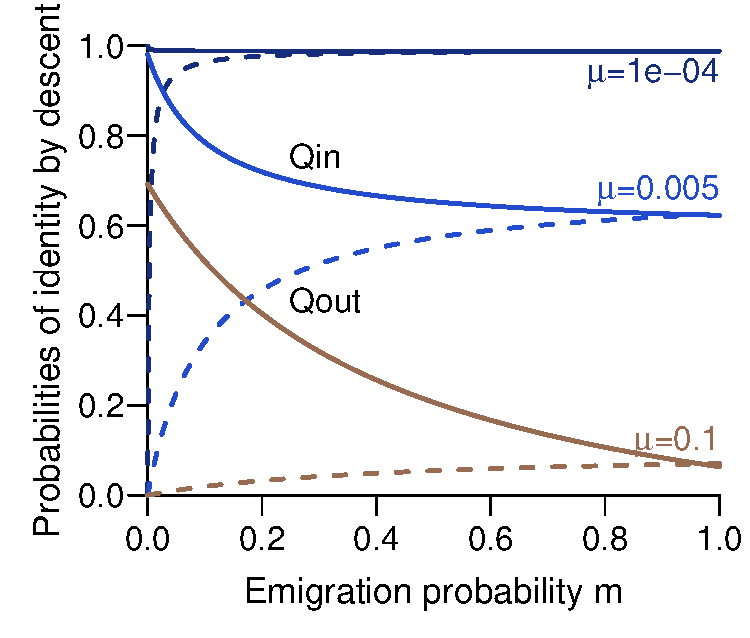
\includegraphics[width = \wpic]{../Programs/R/Pics/QplotM.pdf}}
&
\subfigure[\label{fig:sub:QWF}Wight-Fisher]{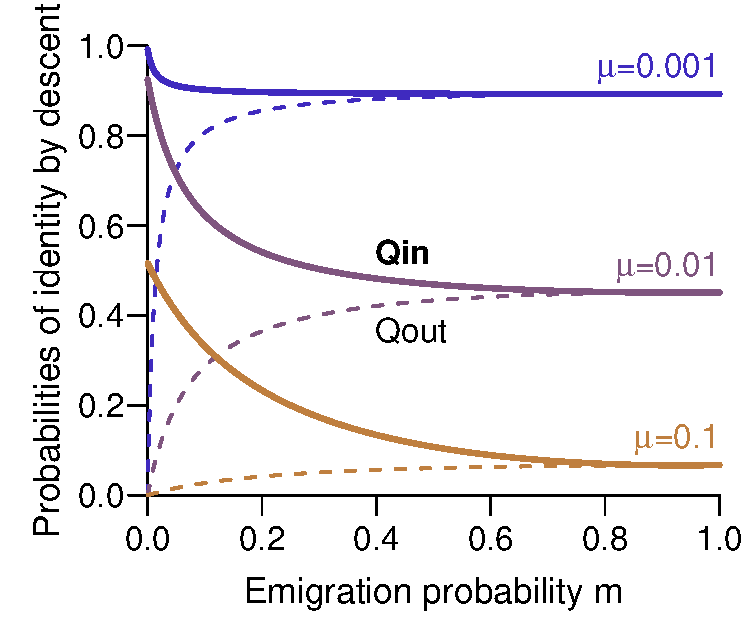
\includegraphics[width = \wpic]{../Programs/R/Pics/QplotWF.pdf}}
\end{tabular}
\caption{Probabilities of identity by descent, for two different individuals within the same deme ($\Qin$, full curves) and two individuals in different demes ($\Qout$, dashed curves), as a function of the emigration probability $m$, for different values of the mutation probability $\mu$ ($0.001$, $0.01$, $0.1$), and for the two types of life-cycles (\subref{fig:sub:QM}: Moran, \subref{fig:sub:QWF}: Wright-Fisher). Other parameters: $n=4$ individuals per deme, $\ndemes = 15$ demes. }
\label{fig:Q}
\end{figure}

\clearpage
\subsection{Expected frequencies of altruists for each life-cycle}

For each of the life-cycles that we consider, the expected frequency of altruists in the population, $\Esp{\overline{X}}$, can be approximated as
\begin{equation}\label{eq:EXapprox}
\Esp{\overline{X}} \approx \mutbias + \omega \frac{\mutbias (1-\mutbias)}{\mu} \left[ \bb \left( \beta_{\direct} - \beta_{\indirect} \right) - \cc \left( \gamma_{\direct} - \gamma_{\indirect} \right) \right].
\end{equation}
(Calculations leading to \eqref{eq:EXapprox} are presented in  \appname~\ref{sec:app:EX}.)\\
The mutation bias $\mutbias$ corresponds to the expected proportion of altruists in the population in the absence of selection (\ie, when $\omega = 0$); $\omega$ is the parameter that scales the effects of interactions between individuals, which is assumed to be small. The subscript $_{\direct}$ refers to ``direct'' effects, and the subscript $_{\indirect}$ to ``indirect'' effects. ``Direct'' effects involve effects on primary beneficiaries of the benefits~($\bb$) and costs~($\cc$) of social interactions \citep{WestGardner2010}, \ie, social interactants (for the benefits $\bb$) and the focal individuals themselves (for the costs $\cc$). ``Indirect'' effects corresponds to effects on secondary interactants, \ie, to (kin) competition. By providing a benefit to a deme-mate and thereby increasing its fecundity, a focal altruist indirectly harms others by reducing their relative fecundity ($\beta_{\indirect}$ term in \eqref{eq:EXapprox}); by having a reduced fecundity due to the cost of altruism, a focal altruist indirectly favors others by increasing their relative fecundity ($\gamma_{\indirect}$ term).

We now present the values of these different terms for the three life-cycles under study.  

\subsubsection{Direct effects}
Direct (/primary) effects are similar for the three life-cycles; the only difference is the value of probabilities of identity by descent $Q$ (as seen in the previous section, they differ between Moran and Wright-Fisher life-cycles):
%
\begin{subequations}\label{eq:directeffects}
\begin{align}
\beta_{\direct}^{\BD} = \beta_{\direct}^{\DB} &= \left( 1-\mu\right) \Qin^{\Moran}, \label{eq:bBDD}\\
\beta_{\direct}^{\WF} &= \left( 1-\mu\right) \Qin^{\WF}; \label{eq:bWFD}\\
%
%
\gamma_{\direct}^{\BD} = \gamma_{\direct}^{\BD} = \gamma_{\direct}^{\WF} &= 1-\mu.\label{eq:cBDD}
\end{align}
\end{subequations}
%
For both benefits and costs, direct effects only count when there is no mutation (hence the ($1-\mu$) factors). 
Direct effects of benefits $\bb$ (\eqref{eq:bBDD} and \eqref{eq:bWFD}) only count if the interaction takes place with an individual who is identical by descent. With the population structure that we consider, social interactions only occur within demes, so only $\Qin$ is present in \eqref{eq:bBDD} and \eqref{eq:bWFD}. On the other hand, the direct effect of the fecundity cost $\cc$ (\eqref{eq:cBDD}) does not depend on the type of interactant, since the same cost $\cc$ is paid by altruists irrespective of the interactant's identity. 

As seen in the previous section, $\Qin^{\Moran}$ and $\Qin^{\WF}$ decrease with the emigration probability $m$ (actually only until $m=\frac{d-1}{d}$ for the latter). Consequently, the magnitude of the direct (beneficial) effects of benefits $\bb$ provided by altruists ($\beta_{\direct}$) decreases when the emigration probability $m$ increases, while the direct (detrimental) effects ($\gamma_{\direct}$) due to the direct cost of altruism $\cc$ are constant. As a result, if we only considered direct effects, we would conclude that more emigration $m$ is detrimental to the evolution of altruistic behaviour. However, there are also indirect effects at play. 

\subsubsection{Indirect effects}
Indirect (/secondary) effects are collateral effects on other individuals; they depend on the type of life-cycle, and always involve individuals who are identical by descent. 

\paragraph{Moran Birth-Death} Changing the fecundity of a focal individual has two kinds of indirect effects on others: \begin{inparaenum}[\it i\rm )]\item it changes their probability of being the one chosen to reproduce -- this affects all individuals in the population who are identical by descent to the focal, and \item it changes their probability of dying because the number of offspring landing in their site changes -- this affects individuals in the population who can send offspring at the same locations as the focal and are identical-by-descent to it. For this life-cycle, the indirect effects are: \end{inparaenum}
%
\begin{subequations}
\begin{equation}\label{eq:bBDI}
\begin{split}
\beta_{\indirect}^{\BD} &=  (1-m) \left(\frac{n-1}{n} \Qin^{\Moran} + \frac{1}{n}\right) + m \, \Qout^{\Moran} %
- \mu \frac{ 1 + (n-1) \Qin^{\Moran} + n (d-1) \Qout^{\Moran}}{n d} \\
&= \gamma_{\indirect}^{\BD}.
\end{split}
\end{equation}
%
(Calculation details are presented in \appname~\ref{sec:app:EX}.)\\
The formulas are the same for the indirect effects associated to $\bb$ and to $\cc$; in other words, the balance between the two indirect effects remains the same when the emigration probability changes. The term $\left(\frac{n-1}{n} \Qin^{\Moran} + \frac{1}{n}\right)$, which will appear again later, corresponds to the probability that two individuals sampled with replacement from the same deme are identical by descent. Indirect effects are indeed also felt by the focal individual itself (\eg, increasing the fecundity of another individual implies decreasing one's own relative fecundity). 

Replacing $\Qin$ and $\Qout$ by their formula for the Moran life-cycle (\eqref{eq:QM}), we conclude that $\beta_{\indirect}^{\BD}=\gamma_{\indirect}^{\BD}$ are decreasing functions of the emigration probability~$m$ (calculations in the supplementary Mathematica file).

\paragraph{Moran Death-Birth} With this life-cycle,  death comes first and every individual in the population has the same survival probability ($1/N$). The indirect consequences of changing a focal individual's fecundity affect all individuals who can send their offspring to the same locations as the focal, and who are identical by descent to it. We obtain
\begin{equation}\label{eq:bDBI}
\begin{split}
\beta_{\indirect}^{\DB} & = (1-\mu ) \Bigg[ \left( \frac{1}{n} + \frac{ (n-1) \Qin^{\Moran} }{n} \right) \left( (1-m)^2 +  \frac{m^2}{ (d-1)} \right) \\ 
%
& \qquad \qquad \quad + \Qout^{\Moran} \, \left(2 m \, (1-m) +  (d-2) \frac{m^2}{(d-1)}\right)  \Bigg] \\
& = \gamma_{\indirect}^{\DB}
%
\end{split}
\end{equation}
The brackets in \eqref{eq:bDBI} contain a sum of two terms. 
The first term corresponds two individuals from the same deme (with replacement) whose offspring either do not emigrate, or emigrate together to the same deme. The second term corresponds to individuals initially from different demes who end up in the same deme (either one of their home demes, or a third deme). 

Here again, $\beta_{\indirect} = \gamma_{\indirect}$, so the balance between indirect benefits and indirect costs does not change when the emigration probability $m$ increases.

Replacing $\Qin$ and $\Qout$ by their formulas given in \eqref{eq:QM}, we can conclude that  $\beta_{\indirect}^{\DB}=\gamma_{\indirect}^{\DB}$ first decreases with the emigration probability $m$, and increases again after a threshold value $m_c'$, which is smaller than $m_c^{\WF}=(d-1)/d$) (calculation details are presented in the supplementary Mathematica file).  

\paragraph{Wright-Fisher} With this life-cycle, generations are synchronous and all individuals again all have the same survival probability (now equal to $0$ at all sites). As a result, the formulas for $\beta_{\indirect}^{\WF}$ and $\gamma_{\indirect}^{\WF}$ are the same as $\beta_{\indirect}^{\DB}$ and $\gamma_{\indirect}^{\WF}$, except that instead of $\Qin^{\Moran}$ and $\Qout^{\Moran}$, we need to use $\Qin^{\WF}$ and $\Qout^{\WF}$ (given in \eqref{eq:QWF}). Once this is done, we see that $\beta_{\indirect}^{\WF} = \gamma_{\indirect}^{\WF}$ first decreases with the emigration probability $m$, and increases again after the threshold value $m_c^{\WF} = (d-1)/d$. This emigration threshold was identified above as the emigration probability such that offspring have an equal chance of landing in their natal deme or in any other deme, \ie, $\din=\dout$ (calculation details are presented in the supplementary Mathematica file.)    
\end{subequations}

\subsection{Identifying threshold values of the mutation probability $\mu$}

In the previous section, we investigated the impact of changes in the emigration probability $m$ on each of the terms that make up the expected frequency of altruists $\Esp{\overline{X}}$. Now we need to combine these different terms to focus on the quantity we are eventually interested in, $\Esp{\overline{X}}$. The rather lengthy formulas that we obtain are relegated to the \appname and supplementary Mathematica file, and we concentrate here on the results. 

\subsubsection{Moran Birth-Death}

For this life-cycle, we find that the expected frequency of altruists $\Esp{\overline{X}}$ is a monotonic function of the emigration probability $m$; the direction of the change depends on the value of the mutation probability $\mu$ compared to a threshold value $\mu_c^{\BD}$. When $\mu<\mu_c^{\BD}$, $\Esp{\overline{X}}$ decreases with $m$, while when $\mu>\mu_c^{\BD}$, $\Esp{\overline{X}}$  increases with $m$. The critical value $\mu_c^{\BD}$ is given by 
\begin{equation}\label{eq:mucBD}
\mu_c^{\BD} = %
1 - \frac{\bb  - \cc + \sqrt{(\bb - \cc) \left(4 \bb (n d)^2 + \bb - \cc \right)} }{2 \bb n d}
\end{equation}
%
This result is illustrated in figure~\ref{fig:EX}\subref{fig:EXBD}; with the parameters of the figure, $\mu_c^{\BD} \approx 0.026$.

\subsubsection{Moran Death-Birth}

The relationship between $\Esp{\overline{X}}$ and $m$ is a bit more complicated for this life-cycle. For simplicity, we concentrate on what happens starting from low emigration probabilities (\ie, the sign of the slope of $\Esp{\overline{X}}$ as a function of $m$ when $m\to 0$). If the benefits $\bb$ provided by altruists are relatively low ($\bb < \cc (n+1)$), $\Esp{\overline{X}}$ initially increases with $m$ provided the mutation probability $\mu$ is greater than a threshold value $\mu_c^{\DB}$ given in \eqref{eq:mucDB} below; otherwise, when the benefits are high enough, $\Esp{\overline{X}}$ initially increases with $m$ for any value of $\mu$. Combining these results, we write
\begin{equation}\label{eq:mucDB}
\mu_c^{\DB} = \begin{cases}
\dfrac{ (n+1) \cc - \bb}{ (2 n - 1) \bb - (n-1) \cc} & \textrm{if $\bb < \cc (n+1)$,} \\
%
0 & \textrm{otherwise. }
\end{cases}
\end{equation} 
%
In figure~\ref{fig:EX}\subref{fig:EXDB}, the parameters are such that $\mu_c^{\DB} = 0$. 

The expected frequency of altruists $\Esp{\overline{X}}$ then reaches a maximum at an emigration probability $m_c^{\DB}$ (whose complicated equation is given in the supplementary Mathematica file), as can be seen in figure~\ref{fig:EX}\subref{fig:EXDB}. When the mutation probability gets close to $0$ ($\mu \to 0$), $m_c^{\DB}$ also gets close to $0$, 

\subsubsection{Wright-Fisher}

The expected frequency of altruists in the population reaches an extremum when $m = m_c^{\WF} = \frac{d-1}{d}$. This extremum is a maximum when the mutation probability is higher than a threshold value $\mu_c^{\WF}$ given by 
\begin{equation}
\mu_c^{\WF} = 1-\sqrt{1-\frac{\cc}{\bb}},
\end{equation}
and it is a minimum otherwise. With the parameters of figure~\ref{fig:EX}\subref{fig:EXWF}, $\mu_c^{\WF} = 0.034$. 

% Figure weak selection
\begin{figure}
\hspace{-2cm}\begin{tabular}{ccc}
\subfigure[Death-Birth \label{fig:EXDB}]{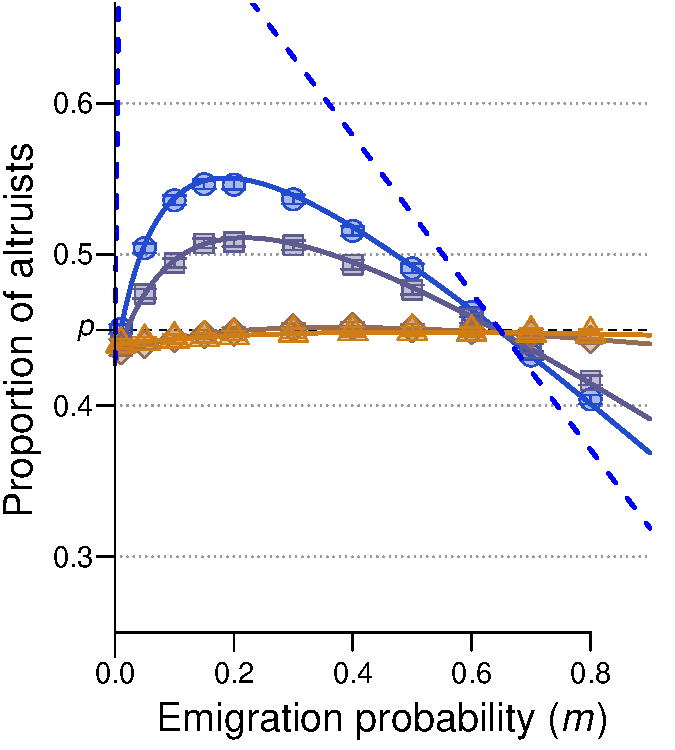
\includegraphics[type=pdf,ext=.pdf,read=.pdf, width=\wpic]{../Programs/R/Pics/EXDB_sel0.005_htg0}}
&
\subfigure[Birth-Death \label{fig:EXBD}]{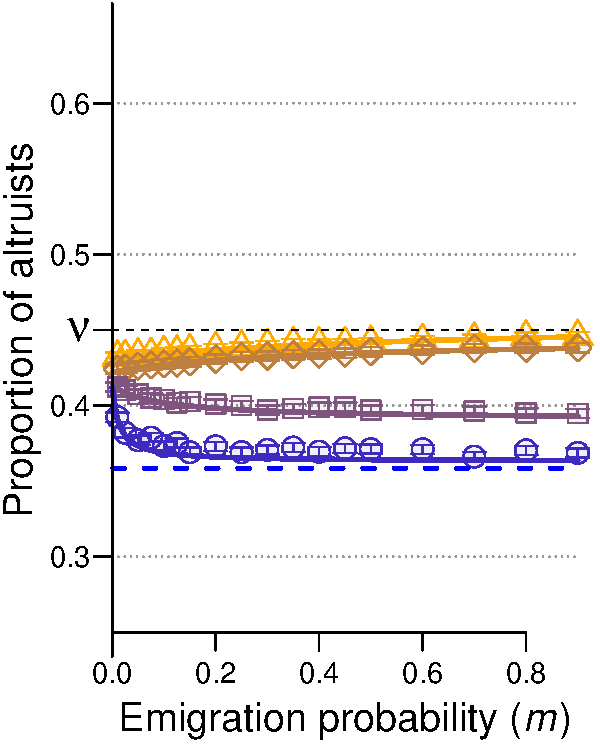
\includegraphics[type=pdf,ext=.pdf,read=.pdf, width=\wpic]{../Programs/R/Pics/EXBD_sel0.005_htg0}}
&
\subfigure[Wright-Fisher \label{fig:EXWF}]{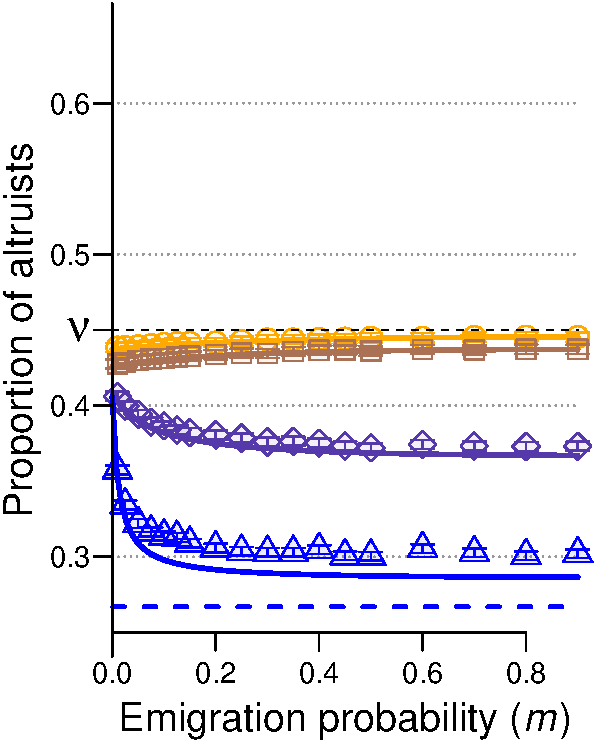
\includegraphics[type=pdf,ext=.pdf,read=.pdf, width=\wpic]{../Programs/R/Pics/EXWF_sel0.005_htg0}}
\end{tabular}
\caption{Expected proportion of altruists under weak selection, as a function of the emigration probability $m$, for different mutation values ($\mu = 0.001$ (blue, dots), $0.01$ (purple, squares), $0.1$ (brown, diamonds), $0.25$ (orange, triangles); the dashed blue lines correspond to $\mu=0$) and different life-cycles (\subref{fig:EXDB} Moran Death-Birth, \subref{fig:EXBD} Moran Birth Death, \subref{fig:EXWF} Wright-Fisher). The curves are the analytical results, the points are the output of numerical simulations. 
Parameters: $\omega = 0.005$, $\mutbias=0.45$, $b = 15$, $c = 1$, $n=4$ individuals per deme, $\ndemes=15$ demes.}
\label{fig:EX}
\end{figure}

\subsection{Relaxing key assumptions}

To derive our analytical results, we had to make a number of simplifying assumptions, such as the fact that selection is weak ($\omega \ll 1$), and the fact that the structure of the population is regular (all demes have the same size $n$). We explored with numerical simulations the effect of relaxing these key assumptions. When selection is strong, the patterns that we identified not only still hold but are even more marked, as shown on  figure~\ref{fig:EXstrongsel}. 

To relax the assumption of equal deme sizes, we randomly drew deme sizes at the beginning of simulations, with sizes ranging from $2$ to $6$ individuals and on average $\overline{n} = 4$ individuals per deme as previously. As shown in figure~\ref{fig:EXhtg}, the patterns initially obtained with a homogeneous population structure are robust when the structure is heterogeneous. 
 
For the Moran model, it may seem odd that an offspring can replace its own parent (which can occur since $d_{ii} \neq 0$). Figure~\ref{fig:EXdself}, plotted with dispersal probabilities preventing immediate replacement of one's own parent (for all sites $i$, $d_{ii}=\dself=0$; $\din = (1-m)/(n-1)$ for two different sites in the same deme, $\dout$ remaining unchanged), confirms that this does affect our conclusions. 

\section{Discussion}
% Summary
\subsection*{The expected frequency of altruists in a subdivided population can increase with the probability of emigration}
Assuming that the transmission of a social strategy (being an altruist or a defector) from a parent to its offspring could be imperfect, we found that the expected frequency of altruists maintained in a population could increase with the probability $m$ of emigration out of the parental deme, a parameter tuning population viscosity. This result can seem surprising, because it contradicts the conclusions obtained under the assumption of nearly perfect strategy transmission (\ie, in the case of genetic transmission, when mutation is very weak or absent). Under nearly perfect strategy transmission indeed, increased population viscosity (\ie, decreased emigration probability) is either neutral \citep[][and dashed lines in figures~\ref{fig:EX}\subref{fig:EXBD}--\subref{fig:EXWF}]{Taylor1992islandmodel} or favorable \citep[][and dashed lines in figure~\ref{fig:EX}\subref{fig:EXDB}]{TaylorDayWild2007} to the evolution of altruistic behavior. 

\subsection*{Quantitative vs. qualitative measures}
% Measure of altruism: quanti vs quali
We used a quantitative measure, the expected frequency of altruists in the population ($\Esp{\overline{X}}$), to explore how non-zero mutation probabilities altered the impact of population viscosity. Often however, evolutionary success is measured qualitatively, by comparing a quantity (an expected frequency, or, in models with no mutation, a probability of fixation) to the value it would have in the absence of selection. In our model, this amounts to saying that altruism is favored whenever $\Esp{\overline{X}} > \mutbias$ ($\mutbias$ is plotted as a horizontal dashed line in figure~\ref{fig:EX}). 
Some of our conclusions change if we switch to this qualitative measure of evolutionary success: Under the Moran Birth-Death and Wright-Fisher life-cycles, population viscosity does not promote the evolution of altruism -- actually, these two life-cycles cannot ever promote altruistic behavior for any regular population structure \citep{Taylor2011}, whichever the probability of mutation \citep{Debarre2017}. 
However, under a Moran Death-Birth life-cycle, altruism can be favored only at intermediate emigration probabilities (figure~\ref{fig:EX}\subref{fig:EXDB}): increased emigration can still favor the evolution of altruism under this qualitative criterion.  

% How to explain the result
\subsection*{The result is due to indirect (/secondary) effects}
To explain how the frequency of altruists can increase with the emigration probability $m$, let us go back to the decomposition of the expected frequency of altruists in the population $\Esp{\overline{X}}$ into different terms (\eqref{eq:EXapprox}). 
For all the life-cycles that we consider, the direct effect of helping others ($\beta_{\direct}$) decreases with emigration $m$, while the direct effect of the cost of helping ($\gamma_{\direct}$) does not change with $m$. 
If we (erroneously) considered only direct effects, we would conclude that the expected proportion of altruists decreases with the emigration probability $m$, because an increase in $m$ reduces the probability that two interactants (two deme-mates in this model) are identical by descent. 
But this explanation ignores indirect, competitive, effects. In the three life-cycles that we considered, $\beta_{\indirect} = \gamma_{\indirect}$, so the overall indirect effects are given by $(-(\bb-\cc) \beta_{\indirect})$. Hence, any increase of $\Esp{\overline{X}}$ with $m$ is driven by $\beta_{\indirect}$. Indirect effects correspond to competition: helping another individual indirectly harms others -- even the individual who is providing help is indirectly harmed. This competition can be diluted by increasing the emigration probability $m$. 
The overall effect of $m$ on the expected frequency of altruists depends on the balance between direct and indirect effects. This balance depends on the fidelity of parent-offspring transmission ($\mu$), in particular because probabilities of identity by descent depend on $\mu$. 

Indirect (secondary) effects are less straightforward to understand than direct (/primary) effects, yet they play a crucial role for social evolution in spatially structured populations. Competition among relatives is for instance behind \citet{Taylor1992}'s cancellation result; similarly, the qualitative differences between the Moran Birth-Death and Moran Death-Birth life-cycles is explained by the different scales of competition that the two life-cycle produce \citep{GrafenArchetti2008, DebarreHD2014}. Secondary effects are also behind the evolution of social behaviors such as spite \citep{WestGardner2010}. 

%  To simplify the explanations, let us consider that the number of demes is large: in this case, $\Qout$ is vanishingly small. Let us also assume that there is no direct cost to being an altruist ($\cc = 0$). 

% Order of limits
\subsection*{How small is small and how large is large?}
Our results were derived under the assumption of weak selection, assuming that the phenotypic difference between altruists and defectors is small ($\delta \ll 0$). We considered any fidelity of transmission (any $\mu$ between $0$ and $1$) and population size. However, most models considering subdivided populations assume nearly perfect strategy transmission ($\mu \to 0$) and infinite population sizes (number of demes $\ndemes \to \infty$). The order in which these limits are taken matters, \ie, one needs to specify how small $\mu$, but also $\omega$, are compared to the inverse size of the population. This remark complements findings by \citet{SampleAllen2017}, who highlighted the quantitative differences between different orders of weak selection and large population limits. 

% Steve Frank and other models
\subsection*{Imperfect transmission and Rebellious Children}
Our model bears resemblance to the Rebellious Child Model by \citet{Frank1997}, who studied the evolution of a vertically transmitted cultural trait in an asexually reproducing population. In \citeauthor{Frank1997}'s model, however, relatedness $r$ is treated as a fixed parameter (as acknowledged in the legend of Figure~7 in \citet{Frank1997}). 
Our model is mechanistic; relatedness $r$ necessarily depends on the mutation probability $\mu$, because probabilities of identity by descent do. 

Mutation was also previously included in models investigating the maintenance of cooperative microorganisms in the presence of cheaters \citep{Brockhurst2007, Frank2010}. In both of these models however, only loss-of-function mutation was considered, which corresponds to setting the mutation bias at $\mutbias=0$ in our model. This means that the all-cheaters state is absorbing; no matter how favored cooperators may otherwise be, in the long run, a finite population will only consist of cheaters. 

\subsection*{Interactions and dispersal graphs}

Compared to graphs classically used in evolutionary graph theory (\eg, regular random graphs, grids), the island model is particular because the interaction graph and the dispersal graph are different: interactions take place only within demes ($\eout = 0$), while offspring can disperse out of their natal deme ($\dout >0$). One may wonder whether our result depends on this difference between the two graphs. Figure~\ref{fig:EXsameDE} shows that the result still holds when the dispersal and interaction graphs are the same. In this figure indeed, we let a proportion $m$ (equal to the dispersal probability) of interactions occur outside of the deme where the individuals live, and set $\dself$, the probability of self replacement, equal to $0$, so that the dispersal and interactions graphs are the same. 

\subsection*{Coevolution of dispersal and social behavior}
This work also raises the question of what would happen if dispersal (\eg, the emigration probability $m$) could evolve as well. Recent work on the topic has shown that under some conditions disruptive selection could take place, leading to a polymorphism between sessile altruists and mobile defectors \citep{Parvinen2013, MullonKL2017bioRxiv}. The assumptions of these studies however  differ from ours in important ways, in that they consider continuous traits and use an adaptive dynamics framework, where, notably, mutations are assumed to be very rare. It remains to be investigated how non-rare and potentially large mutations would affect their result. 


\singlespacing
%%% ___ BIBLIO _____
\clearpage
\bibliographystyle{bibstyle}
\bibliography{bibSCSP}
\doublespacing

\processdelayedfloats

\makeatletter
\efloat@restorefloats
\makeatother


\clearpage
% Start the appendix

%TC:ignore 
% Ignore word count after this point

\appendix
 
% Redefine counters
% Equations
%  Redefine the command that creates the equation number.
\renewcommand{\theequation}{\thesection.\arabic{equation}}
%  Reset the counter
\setcounter{equation}{0}  % reset counter
 
% Figures
%  Redefine the command that creates the figure number: adds an S.
\renewcommand{\thefigure}{S\arabic{figure}}
%  Reset the counter  
\setcounter{figure}{0}

% Tables
\renewcommand{\thetable}{S\arabic{table}}
%  Reset the counter  
\setcounter{table}{0}
\section*{Supplementary figures} 

% Figure strong selection
\begin{figure}[h!]
\begin{tabular}{ccc}
\subfigure[Death-Birth]{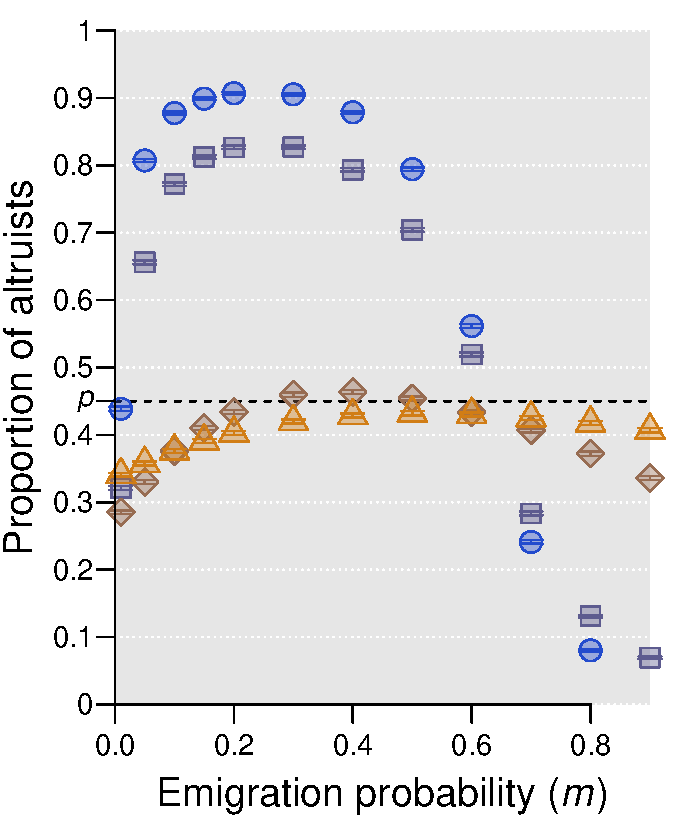
\includegraphics[type=pdf,ext=.pdf,read=.pdf, width=\wpic]{../Programs/R/Pics/EXDB_sel0.1_htg0}}
&
\subfigure[Birth-Death]{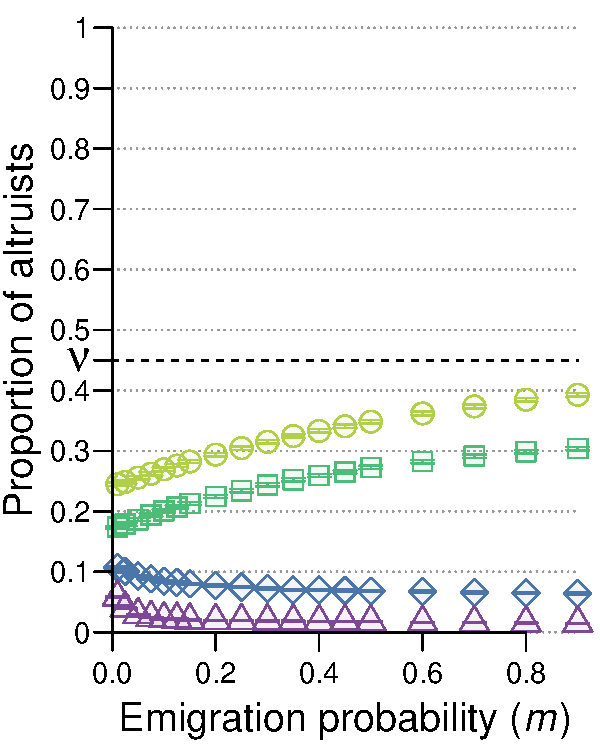
\includegraphics[type=pdf,ext=.pdf,read=.pdf, width=\wpic]{../Programs/R/Pics/EXBD_sel0.1_htg0}}
&
\subfigure[Wright-Fisher]{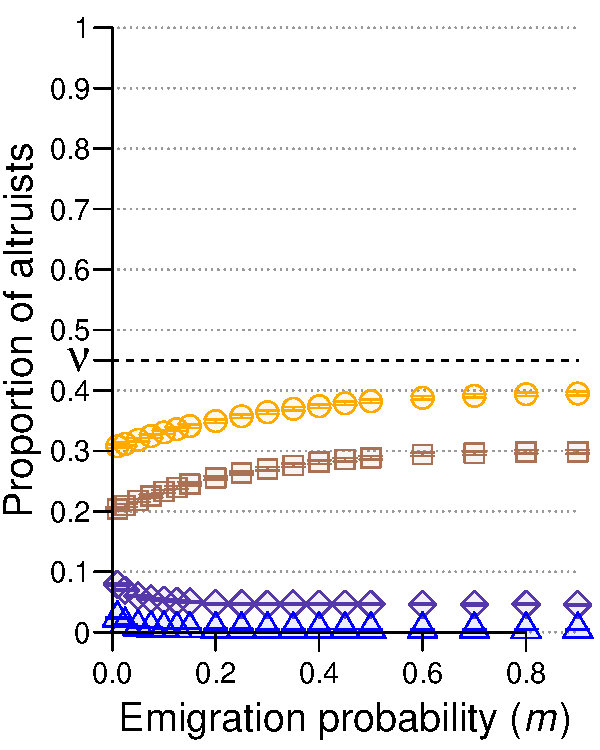
\includegraphics[type=pdf,ext=.pdf,read=.pdf, width=\wpic]{../Programs/R/Pics/EXWF_sel0.1_htg0}}
\end{tabular}
\caption{Equivalent of figure~\ref{fig:EX} (simulations only) but with strong selection ($\omega = 0.1$); please note the change of scale on the vertical axis. All other parameters and legends are identical to those of figure~\ref{fig:EX} (increasing mutation probabilities from blue dots to orange triangles). }
\label{fig:EXstrongsel}
\end{figure}

% Figure heterogeneous population
\begin{figure}
\begin{tabular}{ccc}
\subfigure[Death-Birth]{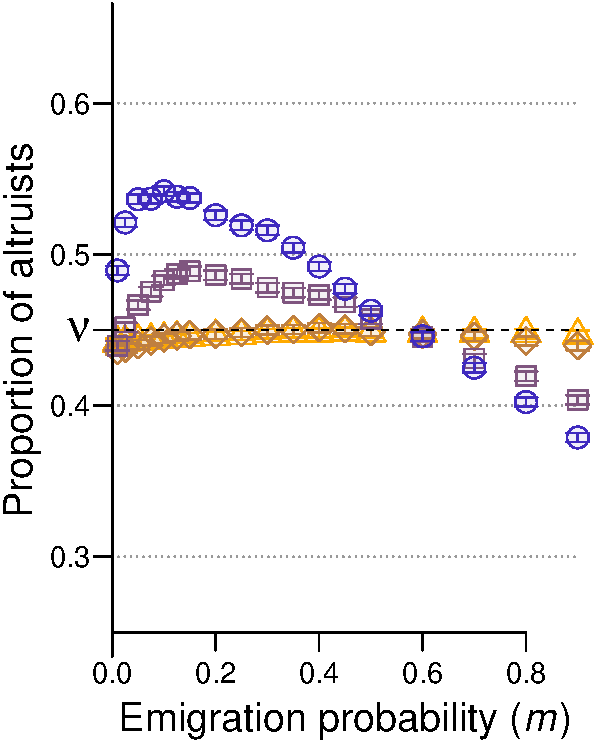
\includegraphics[type=pdf,ext=.pdf,read=.pdf, width=\wpic]{../Programs/R/Pics/EXDB_sel0.005_htg1}}
&
\subfigure[Birth-Death]{
\includegraphics[type=pdf,ext=.pdf,read=.pdf, width=\wpic]{../Programs/R/Pics/EXBD_sel0.005_htg1}}
&
\subfigure[Wright-Fisher]{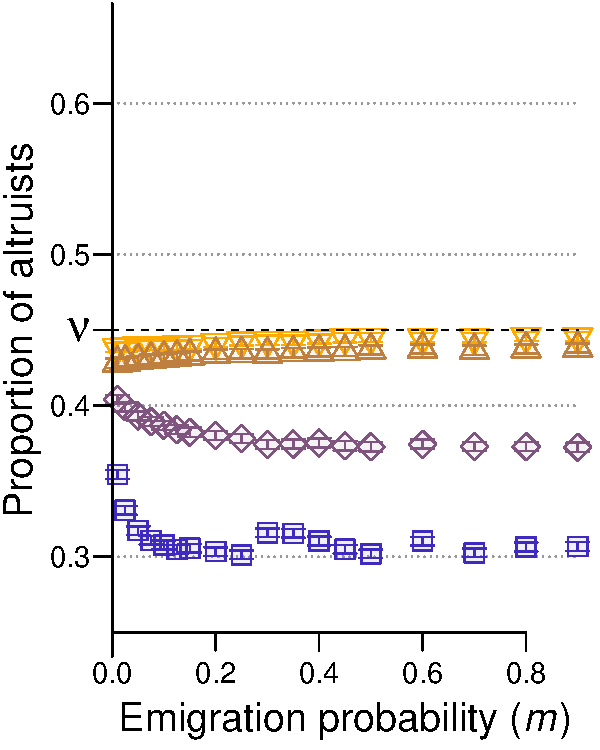
\includegraphics[type=pdf,ext=.pdf,read=.pdf, width=\wpic]{../Programs/R/Pics/EXWF_sel0.005_htg1}}\end{tabular}
\caption{Equivalent of figure~\ref{fig:EX} (simulations only) but with a heterogeneous population structure: deme sizes range form $1$ to $5$ individuals per deme, the average deme size is $4$ as in figure~\ref{fig:EX};  all other parameters and legend are identical to those of figure~\ref{fig:EX}. }
\label{fig:EXhtg}
\end{figure}


 
%\clearpage
%% Figure heterogeneous population
%\begin{figure}
%\begin{tabular}{ccc}
%\subfigure[Death-Birth]{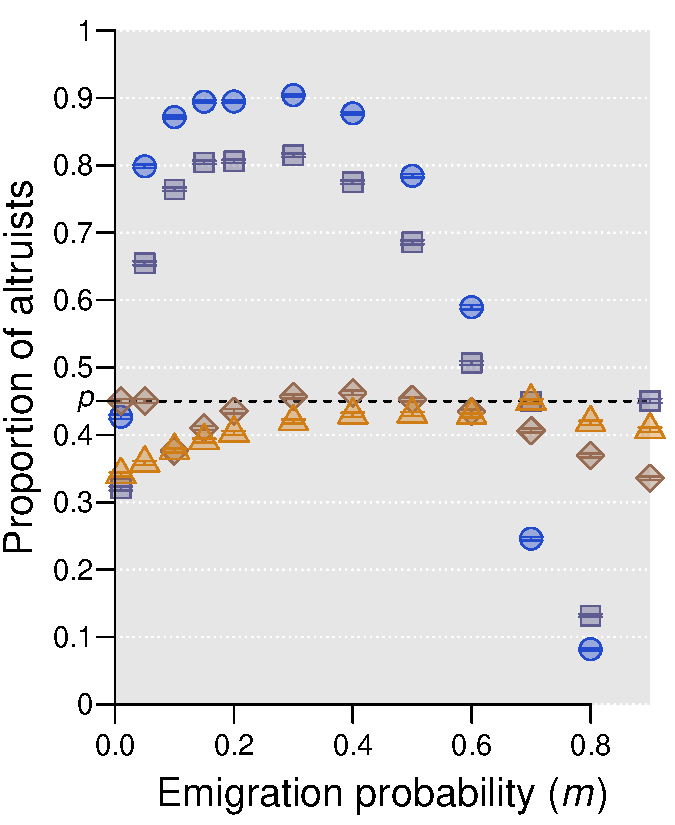
\includegraphics[type=pdf,ext=.pdf,read=.pdf, width=\wpic]{../Programs/R/Pics/EXDB_sel0.1_htg1}}
%&
%\subfigure[Birth-Death]{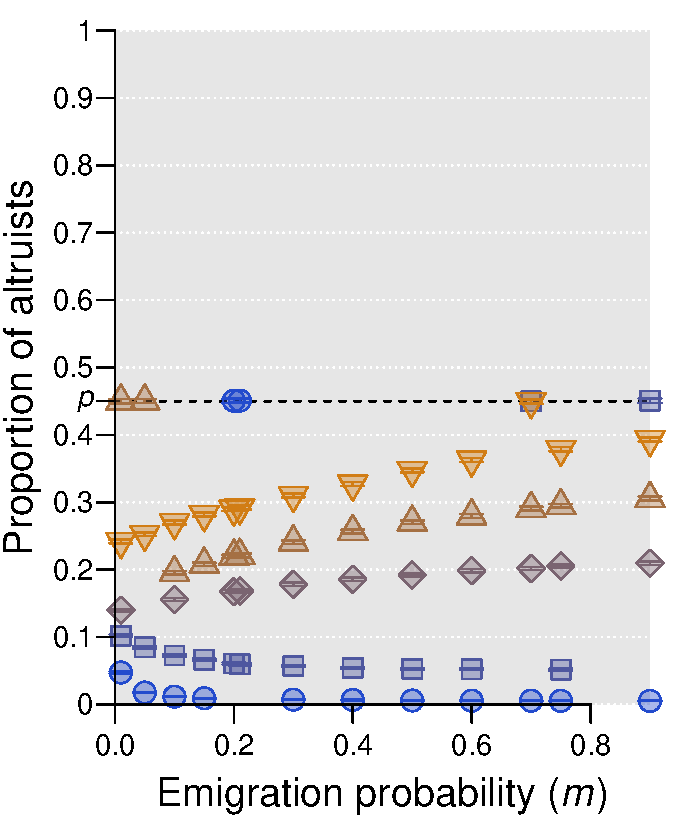
\includegraphics[type=pdf,ext=.pdf,read=.pdf, width=\wpic]{../Programs/R/Pics/EXBD_sel0.1_htg1}}
%&
%\subfigure[Wright-Fisher]{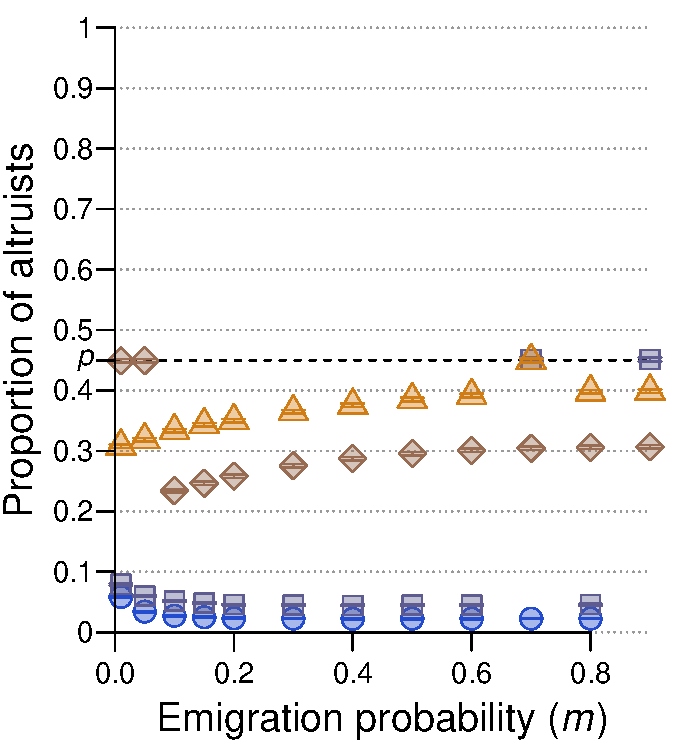
\includegraphics[type=pdf,ext=.pdf,read=.pdf, width=\wpic]{../Programs/R/Pics/EXWF_sel0.1_htg1}}\end{tabular}
%\caption{Strong selection, heterogeneous population}
%\label{fig:island_htgpop}
%\end{figure}



% Figure dself = 0
\begin{figure}
\begin{tabular}{ccc}
\subfigure[Death-Birth \label{fig:EXdselfDB}]{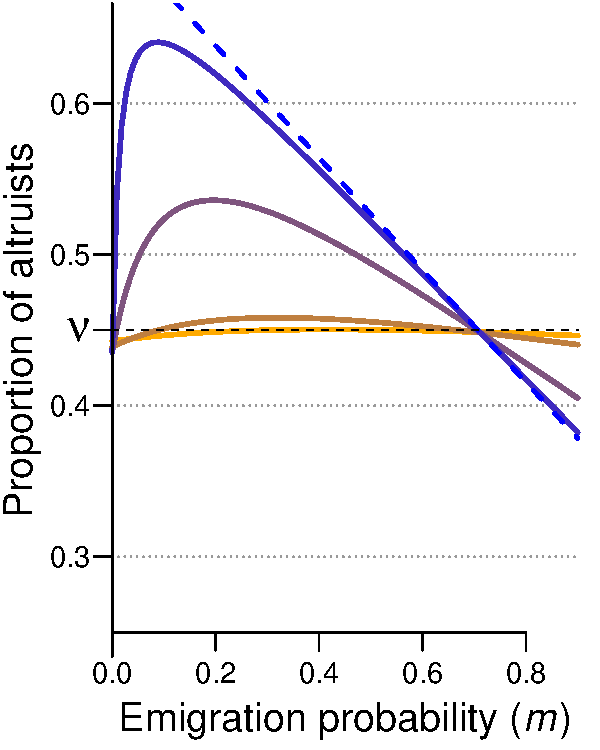
\includegraphics[type=pdf,ext=.pdf,read=.pdf, width=\wpic]{../Programs/R/Pics/EXDB_sel0.005_htg0_nodself}}
&
\subfigure[Birth-Death \label{fig:EXdselfBD}]{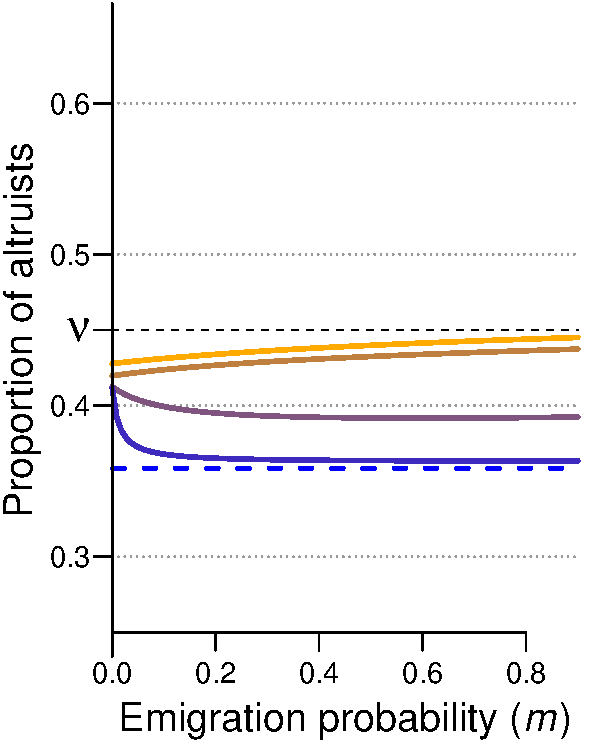
\includegraphics[type=pdf,ext=.pdf,read=.pdf, width=\wpic]{../Programs/R/Pics/EXBD_sel0.005_htg0_nodself}}
&
\subfigure[Wright-Fisher \label{fig:EXdselfWF}]{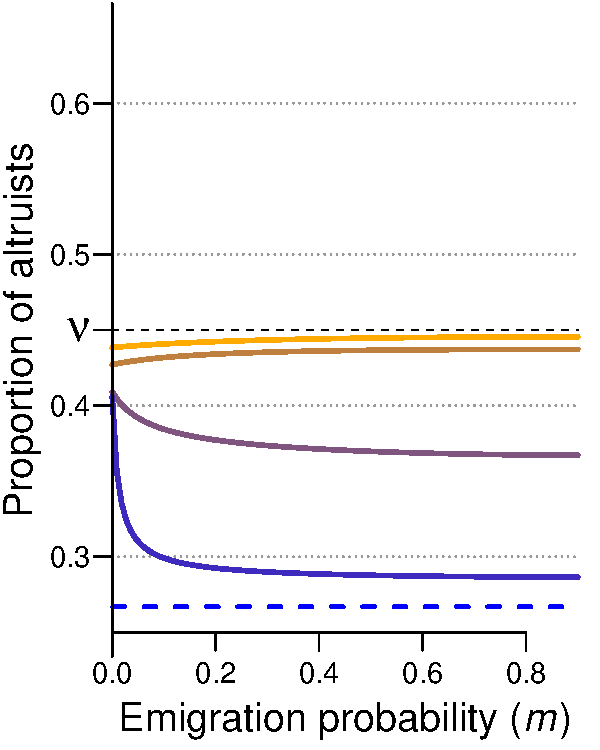
\includegraphics[type=pdf,ext=.pdf,read=.pdf, width=\wpic]{../Programs/R/Pics/EXWF_sel0.005_htg0_nodself}}
\end{tabular}
\caption{Equivalent of figure~\ref{fig:EX} (analysis only), with no self-replacement ($d_{ii} = \dself = 0$ for all sites). }
\label{fig:EXdself}
\end{figure}

% Figure SameDE
\begin{figure}
\begin{tabular}{ccc}
\subfigure[Death-Birth \label{fig:EXsameDEDB}]{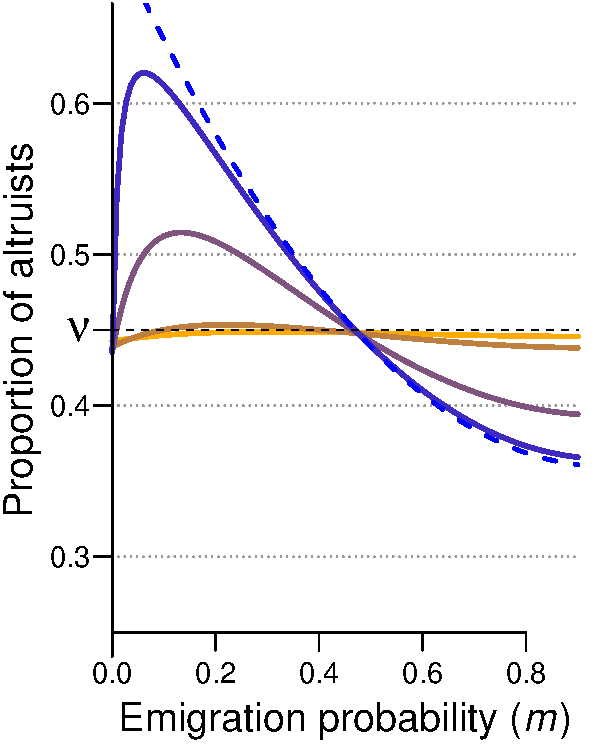
\includegraphics[type=pdf,ext=.pdf,read=.pdf, width=\wpic]{../Programs/R/Pics/EXDB_sel0.005_htg0_nodself_sameDE}}
&
\subfigure[Birth-Death \label{fig:EXsameDEBD}]{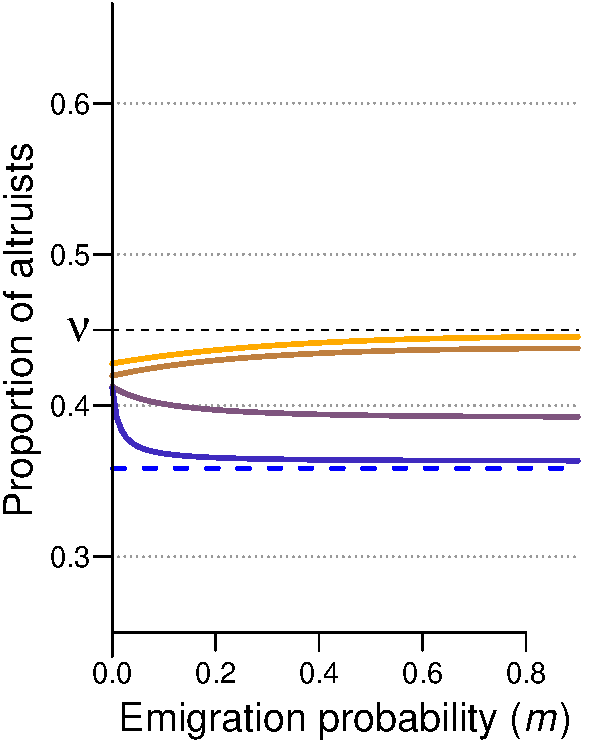
\includegraphics[type=pdf,ext=.pdf,read=.pdf, width=\wpic]{../Programs/R/Pics/EXBD_sel0.005_htg0_nodself_sameDE}}
&
\subfigure[Wright-Fisher \label{fig:EXsameDEWF}]{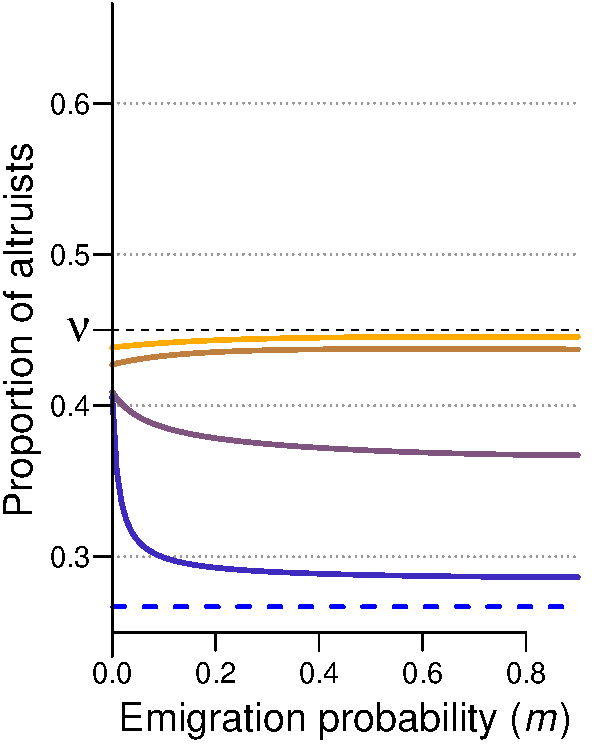
\includegraphics[type=pdf,ext=.pdf,read=.pdf, width=\wpic]{../Programs/R/Pics/EXWF_sel0.005_htg0_nodself_sameDE}}
\end{tabular}
\caption{Equivalent of figure~\ref{fig:EX} (analysis only), with equal dispersal and interaction graphs (\ie, no self-replacement [$d_{ii} = \dself = 0$ for all sites], and a proportion~$m$ of the interactions occurring outside of the home deme). }
\label{fig:EXsameDE}
\end{figure}

\clearpage
\section*{Supplementary Table}

\begin{table}[h!]
\begin{tabular}{>{$}c<{$} l}
\bb & Fecundity benefit given by altruists to social interactants\\
\cc & Fecundity cost paid by altruists\\
d_{ij} & Dispersal probability from site $i$ to site $j$\\
e_{ij} & Interaction probability from site $i$ to site $j$ \\
n & Deme size\\
\ndemes & Number of demes \\
N & Total population size ($N = \ndemes n$) \\
m & Emigration probability\\
Q_{ij} & (Long-term) Probability of identity by descent of individuals at sites $i$ and $j$\\
X_i & Indicator variable, equal to $1$ if site $i$ is occupied by an altruist, to $0$ otherwise (r.v.)\\
\overline{X} & Frequency of altruists in the population (r.v.)\\
\beta & Term associated to the benefits $\bb$\\
\gamma & Term associated to the costs $\cc$ \\
\mu & Mutation probability\\
\mutbias & Mutation bias: probability that mutant is altruist\\
\omega & Parameter scaling the relative effect of social interactions on fecundity\\
\hline
\small \direct & Subscript corresponding to direct/primary effects\\
\small \indirect & Subscript corresponding to indirect/secondary effects\\
\small{\inn} & Subscript used when $i\neq j$ and the two sites are in the same deme\\
\small{\out} & Subscript used when the two sites $i$ and $j$ are in different demes\\
\small{\self} & Subscript used when $i=j$\\
\hline
\small{\BD} & Superscript corresponding to the Moran Birth-Death model\\
\small{\DB} & Superscript corresponding to the Moran Death-Birth model\\
\small{\Moran} & Superscript corresponding to a Moran model\\
\small{\WF} & Superscript corresponding to the Wright-Fisher model
\end{tabular}
\caption{List of symbols. ``r.v.'' means \textit{random variable}. }
\label{tab:symbols}
\end{table}
\clearpage

% Start the appendix
\appendix
 
% Redefine counters
% Equations
%  Redefine the command that creates the equation number.
\renewcommand{\theequation}{\thesection.\arabic{equation}}
%  Reset the counter
\setcounter{equation}{0}  % reset counter
 
%
\begin{center}
{\color{seccol}{\LARGE \bfseries \appname}}
\end{center}

\pagestyle{appendix}
\singlespace


\section{Expected frequency of altruists\label{sec:app:EX}}

\textit{Note: The calculation steps are the same as the ones presented in \citet{Debarre2017}; they are presented here so that the article is self-contained, but there are no new results in \appname~\ref{sec:app:EX}. }

In this section, we work with a generic regular population structure (with symmetries such that all individuals behave the same way in expectation), of which the island model is a particular case. 

\subsection{For a generic life-cycle \label{sec:app:generic}}

We want to compute the expected proportion of altruists in the population. We represent the state of the population at a given time $t$ using indicator variables $X_i(t)$, $1\leq i \leq N$, equal to~$1$ if the individual living at site $i$ at time $t$ is an altruist, and equal to~$0$ if it is a defector; these indicator variables are gathered in a $N$-long vector $\mathbf{X}(t)$. The set of all possible population states is $\Omega = \{0,1\}^N$. The proportion of altruists in the population is written $\overline{X}(t) = \sum_{i=1}^N X_i(t)$. We denote by $B_{ji}(X(t), \omega)$, written $B_{ji}$ for simplicity, the probability that the individual at site $j$ at time $t+1$ is the newly established offspring of the individual living at site $i$ at time $t$. We denote by $D_{i}(X(t), \omega)$ ($D_i$ for simplicity) the probability that the individual living at site $i$ at time $t$ has been replaced (\ie, died) at time $t+1$. Both quantities depend on the chosen life-cycle and on the state of the population; they are given in table~\ref{tab:BD} for each of the life-cycles that we consider. 

\begin{table}[h!]
{
\tabulinesep=1.65mm
\begin{tabu}{lcc}
\hline
Life-cycle & $B_{ij}$ & $D_i$ \\   
\hline
%
Moran Birth-Death & %
$d_{ji} \dfrac{\myphantom f_{j} \myphantom}{\sum_{k =1}^N f_{k}}$  & %
$\dfrac{\myphantom \sum_{j=1}^N d_{ji} f_j\myphantom }{\sum_{k=1}^N f_k}$ \vspace{0.em}\\
%
%
Moran Death-Birth & %
$\dfrac{1}{N}\dfrac{ d_{ji} f_j }{\sum_{k=1}^N d_{ki} f_k}$ & %
$\dfrac{1}{N}$ \vspace{0.em}
\\
%
%
Wright-Fisher & %
$\dfrac{d_{ji} f_j}{\sum_{k=1}^N d_{ki} f_k}$ & $1$
\end{tabu}
}
\caption{Formulas of $B_{ij}$ and $D_{i}$ for each of the life-cycles that we consider; $f_i$ (shorthand notation for $f_i(X, \omega)$) is the fecundity of the individual living at site $i$, as defined in \eqref{eq:deff}. }
\label{tab:BD}
\end{table}
Since a dead individual is immediately replaced by one new individual, 
\begin{subequations}
\begin{equation}\label{eq:DBequiv}
D_i = \sum_{j=1}^N B_{ij}
\end{equation}
holds for all sites $i$. The structure of the population is also such that in the absence of selection ($\omega = 0$, so that $f_i=1$ for all sites $1\leq i\leq N$), all individuals have the same probability of dying and the same probability of having successful offspring (\ie, of having offspring that become adults at the next time step), so that
\begin{equation}\label{eq:DBRV}
D_i^0 = \sum_{j=1}^N B_{ji}^0 = B^*, 
\end{equation}
where the $^0$ subscript means that the quantities are evaluated for $\omega = 0$. This also implies that $B_{ij}^0$ and $D_i^0$ do not depend on the state $\mathbf{X}$ of the population. For the Moran life-cycles, $B^*=1/N$, while for the Wright-Fisher life-cycle, $B^*=1$. 
(The difference between \eqref{eq:DBRV} and  \eqref{eq:DBequiv} is that we are now considering offspring produced by $i$ landing on $j$).

\end{subequations}


Given that the population is in state $\mathbf{X}(t)$ at time $t$, the expected frequency of altruists at time $t+1$ is given by
\begin{subequations}
\begin{equation}\label{eq:conditionalchange}
\Esp{\overline{X}(t+1) | \mathbf{X}(t)} = %
\frac{1}{N} \sum_{i=1}^N \left[ \sum_{j=1}^N B_{ij} \left( X_j (1-\mu) + \mu \mutbias \right) + (1-D_i) X_i \right]. 
\end{equation}
\end{subequations}
The first term within the brackets corresponds to births: the type of the individual living at $i$ at time $t+1$ depends on the type of its parent (living at site $j$), and on whether mutation occurred. The second term in the brackets of \eqref{eq:conditionalchange} corresponds to the survival of the individual living at site $i$. 

Given that there is no absorbing population state (a lost strategy can always be recreated by mutation), there is a stationary distribution of population states; the expected frequency of altruists does not change anymore for large times~$t$ (realized frequencies of course keep changing). We denote by $\xi(\mathbf{X}, \omega, \mu)$ the probability that the population is in state $\mathbf{X}$, given the strength of selection $\omega$ and the mutation probability $\mu$. Taking the expectation of \eqref{eq:conditionalchange} ($\Esp{\overline{X}} = \sum_{X \in \Omega} \overline{X}\xi(\mathbf{X}, \omega, \mu)$), we obtain, after reorganizing:
\begin{equation}\label{eq:statdist}
0 = \frac{1}{N} \sum_{X\in \Omega} \sum_{i=1}^N \left[ \sum_{j=1}^N B_{ij} \left( X_j (1-\mu) + \mu \mutbias \right) -D_i X_i \right] \xi(\mathbf{X}, \omega, \mu). 
\end{equation}

Now, we use the assumption of weak selection ($\omega \ll 1$) and consider the first-order expansion of \eqref{eq:statdist} for $\omega$ close to $0$. First, we note that in the absence of selection ($\omega = 0$), the population is at a mutation-drift balance; the expected state of every site $i$ is then $\Espzero{X_i} = \sum_{X\in \Omega} X_i \xi(X, 0, \mu)= \mutbias$ (recall that $\mutbias$ is the mutation bias parameter). Secondly, we further expand derivatives of $B_{ji}$ and $D_i$ thanks to the chain rule, using the variables $f_k$ ($1\leq k \leq N$), corresponding to individual fecundities (also, recall that $f_k=1$ when $\omega=0$). Thirdly, we note that for all the life-cycles that we consider, the total number of deaths in the population during one time step does not depend on population composition (it is exactly $1$ death for the Moran life-cycles, and exactly $N$ for the Wright-Fisher life-cycle), so that $\sum_{i,j=1}^N B_{ij}$ does not depend on $\omega$. 
After simplification and reorganization, the first order expansion of \eqref{eq:statdist} yields
%
%
\begin{equation}\label{eq:weaksel1}
\begin{split}
0 =&  \frac{1}{N}  \sum_{i,k=1}^N \Bigg[  \derivvv{\left(\sum_{j=1}^N (1-\mu) B_{ji}  - D_i \right)}{f_k}{f_k=1}  \\ 
%
&  \qquad \qquad \times \left( \sum_{\ell =1}^N e_{\ell k} \bb \sum_{X\in \Omega} X_{\ell} X_i \xi(\mathbf{X}, 0, \mu) - \cc \sum_{X\in \Omega} X_k X_i \xi(\mathbf{X}, 0, \mu) \right)  \Bigg] \\ 
%
%&- \frac{\mu }{N} \sum_{X\in \Omega} \sum_{i, k=1}^N   \derivvv{\sum_{j=1}^N B_{ji}}{f_k}{f_k=1} \left( \sum_{\ell =1}^N e_{\ell k} X_{\ell} X_i - \cc X_k X_i\right)   \xi(\mathbf{X}, 0, \mu) \\ 
%
%& + \frac{1}{N} \sum_{X\in \Omega} \sum_{i=1}^N \left[ \sum_{j=1}^N B_{ji}^0 X_i  -D_i^0 X_i \right] \deriv{\xi(\mathbf{X}, \omega, \mu)}{\omega} 
%
& - B^* \mu \derivv{\Esp{\overline{X}}}{\omega}{\omega} 
%
+ \bigO{\omega^2}. 
\end{split}
\end{equation}
The terms $\sum_{X\in\Omega} X_i X_j \xi(\mathbf{X}, 0, \mu)$, that we will denote by $P_{ij}$, correspond to the expected state of the pair of sites ($i$, $j$), evaluated in the absence of selection ($\omega = 0$). We can also replace these terms by 
\begin{equation}\label{eq:QP}
P_{ij} = \mutbias^2 + \mutbias (1-\mutbias) Q_{ij}.
\end{equation}
%
In \appname~\ref{sec:app:IBD}, we will see that recursions on $P_{ij}$ reveal that $Q_{ij}$ can be interpreted as a probability of identity by descent, \ie, the probability that the individuals at sites $i$ and $j$ have a common ancestor and that no mutation has occurred on either lineage since the ancestor. 

Finally, we obtain a first-order approximation of the expected frequency of altruists in the population with 
\begin{equation}\label{eq:EXgeneric}
\Esp{\overline{X}} = \mutbias + \omega \,  \derivv{\Esp{\overline{X}}}{\omega}{\omega} + \bigO{\omega^2},
\end{equation}
where $\derivv{\Esp{\overline{X}}}{\omega}{\omega}$ is obtained from \eqref{eq:weaksel1}. We then need to replace the $B_{ij}$ and $D_{j}$ terms by their formulas for each life-cycle (given in table~\ref{tab:BD}), and the $d_{ij}$ and $e_{ij}$ terms by their formulas (given in \eqref{eq:defD}) and \eqref{eq:defE}, respectively). For each life-cycle we can group terms as
\begin{equation}
\derivv{\Esp{\overline{X}}}{\omega}{\omega} 
\approx 
\frac{\mutbias (1-\mutbias)}{\mu} \left[ \bb \, (\beta_{D} - \beta_{I}) - \cc \, (\gamma_{D} - \gamma_{I}) \right],
\end{equation}
%
where $\direct$ terms come from the numerators of $B_{ij}$ and $D_i$, and $\indirect$ terms come from the denominator of $B_{ij}$ and $D_i$; replacing $B_{ij}$ and $D_i$ by their formulas given in table~\ref{tab:BD}, we obtain the following sets of equations for each life-cycle:

\paragraph{Moran Birth-Death}
\begin{subequations}\label{eq:EXBDsums}
\begin{align}
\beta_{\direct}^{\BD} &= \sum_{k,\ell=1}^N \frac{1-\mu}{N} e_{k\ell} \, Q_{\ell k}^{\Moran},\\
%
\beta_{\indirect}^{\BD} &= \sum_{j,k,\ell=1}^N \left(  \frac{d_{\ell j}}{N } - \frac{\mu}{N^2}  \right)e_{k\ell} \, Q_{jk}^{\Moran},\\
%
\gamma_{\direct}^{\BD} &= 1-\mu,\\
%
\gamma_{\indirect}^{\BD} &= \sum_{j,k=1}^N \left(  \frac{d_{kj}}{N } - \frac{\mu}{N^2}   \right) \, Q_{jk}^{\Moran} .
\end{align}
\end{subequations}

\paragraph{Moran Death-Birth}\label{eq:EXDBsums}
\begin{subequations}
\begin{align}
\beta_{\direct}^{\DB} &= \sum_{k,\ell=1}^N \frac{1-\mu}{N} e_{k\ell} \, Q_{\ell k}^{\Moran},\\
%
\beta_{\indirect}^{\DB} &= (1-\mu) \sum_{i,j,k,\ell=1}^{N} \frac{ d_{ji} d_{\ell i}}{N}   e_{k\ell} \, Q_{jk}^{\Moran}, \\ 
%
\gamma_{\direct}^{\DB} &= 1-\mu,\\
%
\gamma_{\indirect}^{\DB} &= (1-\mu)\sum_{i,j,k=1}^N  \frac{ d_{ji} d_{ki}}{N }  \, Q_{jk}^{\Moran}.
\end{align}
\end{subequations}

\paragraph{Wright-Fisher}
\begin{subequations}\label{eq:EXWFsums}
\begin{align}
\beta_{\direct}^{\WF} &= \sum_{k,\ell=1}^N \frac{1-\mu}{N} e_{k\ell} \, Q_{\ell k}^{\WF},\\
%
\beta_{\indirect}^{\WF} &= (1-\mu) \sum_{i,j,k,\ell=1}^{N} \frac{ d_{ji} d_{\ell i}}{N}   e_{k\ell} \, Q_{jk}^{\WF}, \\ 
%
\gamma_{\direct}^{\WF} &= 1-\mu,\\
%
\gamma_{\indirect}^{\WF} &= (1-\mu)\sum_{i,j,k=1}^N  \frac{ d_{ji} d_{ki}}{N }  \, Q_{jk}^{\WF}.
\end{align}
\end{subequations}
\Sysref{eq:EXWFsums} is the same set of equations as for the Moran Death-Birth model (\sysref{eq:EXDBsums}), except for the values of probabilities of identity by descent\dots that we now need to compute.  

\subsection{Probabilities of identity by descent\label{sec:app:IBD}}

Here we show the link between the expected state of a pair of sites $P_{ij}$ and probabilities of identity by descent $Q_{ij}$. In our derivation of $\Esp{\overline{X}}$, $P_{ij}$ is the quantity that appears, but most studies use $Q_{ij}$. Both are evaluated in the absence of selection ($\omega = 0$). 

\subsubsection{Moran model}
In a Moran model, exactly one individual dies and one individual reproduces during one time step. Given a state $\mathbf{X}$ at time $t$, at time $t+1$ both sites $i$ and $j\neq i$ are occupied by altruists, if \begin{inparaenum}[\it i\rm)]\item it was the case at time $t$ and neither site was replaced by a non-altruist (first term in \eqref{eq:app:PijM1}), or \item if exactly one of the two sites was occupied by a non-altruist at time $t$, but the site was replaced by an altruist (second and third terms of \eqref{eq:app:PijM1}): \end{inparaenum}
%
\begin{align}\label{eq:app:PijM1}
 \Esp{X_iX_j(t+1)|X(t)=\mathbf{X}} = & X_i X_j \left(1 - \sum_{k=1}^N \frac{1}{N} \left( d_{ki} + d_{kj} \right) \left( (1-X_k) (1-\mu) + \mu (1-\mutbias)\right) \right) \nonumber \\
  &+ X_i (1-X_j) \sum_{k=1}^N \frac{1}{N} d_{kj} \left( X_k (1-\mu) + \mu \mutbias \right)  \\
& + X_j (1-X_i) \sum_{k=1}^N \frac{1}{N} d_{ki} \left( X_k (1-\mu) + \mu \mutbias \right). \nonumber
\end{align}

We take the expectation of this quantity, and consider that the stationary distribution is reached ($t\to \infty$); then $\Esp{X_iX_j(t+1)} = \Esp{X_i X_j (t)}$, and we obtain
%
\begin{equation}\label{eq:app:PijM}
P_{ij} = \frac{1}{2} \left(\sum_{k=1}^N (1-\mu) \left( d_{kj} P_{ki} + d_{ki} P_{kj}\right) \right) + \mu \mutbias^2 \qquad (i\neq j ),
\end{equation} 
while $P_{ii}=\mutbias$. 

Now we substitute $P_{ij} = \mutbias^2 + \mutbias (1-\mutbias) Q_{ij}$ in \eqref{eq:app:PijM}, we obtain
\begin{equation}\label{eq:app:QijM}
Q_{ij} = \frac{1}{2} \sum_{k=1}^N (1-\mu) \left( d_{ki} Q_{kj} + d_{kj} Q_{ki}\right),
\end{equation}
and we realize that $Q_{ij}$ is the probability that the individuals at sites $i$ and $j \neq i$ are identical by descent. To compute it indeed, we need to pick which site was last updated (equal probabilities), then who was the parent ($k$); the other individual needs to be identical by descent to the parent, and no mutation should have occurred ($1-\mu$). 

\subsubsection{Wright-Fisher model}

In a Wright-Fisher model, all individuals are replaced at each time step, so we directly consider the state of the parents:
\begin{align}\label{eq:app:PijWF1}
 \Esp{X_iX_j(t+1)|X(t)=\mathbf{X}} = & \sum_{k, \ell = 1}^N  d_{ki} d_{\ell j} \Bigg( X_k X_{\ell} (1-\mu+\mu \mutbias)^2 \nonumber\\ & \qquad + \left( X_k (1-X_{\ell}) + (1-X_k) X_{\ell} \right) (1-\mu+\mu \mutbias) (\mu \mutbias) \nonumber\\
 & \qquad + (1-X_k)(1-X_{\ell}) (\mu \mutbias)^2 \Bigg)
 %
% = & \sum_{k, \ell = 1}^N  d_{ki} d_{\ell j} \Big(\left( X_k X_{\ell} (1-\mu)^2  \right)+ (2-\mu)\mu \mutbias^2 \Big).
\end{align}
The first term of \eqref{eq:app:PijWF1} corresponds to both parents being altruists, and having altruist offspring; the second line corresponds to exactly one parent being altruist, and the third line to both parents being non-altruists (in this latter case, the two offspring have to be both mutants to be altruists). \\
Taking the expectation and simplifying, we obtain
\begin{equation}\label{eq:app:PijWF}
P_{ij} = \sum_{k, \ell = 1}^N \left( P_{kl} (1-\mu)^2  \right)+ (2-\mu)\mu \mutbias^2. 
\end{equation}
Replacing $P_{ij}$ by $\mutbias^2 + \mutbias (1-\mutbias) Q_{ij}$, \eqref{eq:app:PijWF} becomes
\begin{equation}\label{eq:app:QijWF}
Q_{ij} = \sum_{k, \ell=1}^N d_{ki} d_{\ell j} Q_{k\ell} (1-\mu)^2. 
\end{equation}
Again, $Q_{ij}$ corresponds to a probability of identity by descent: the individuals at sites $i$ and $j$ are identical by descent if their parents were and if neither mutated ($(1-\mu)^2$). 

\clearpage
\section{\label{sec:app:subdiv}In a subdivided population}

\subsection{\label{sec:app:bcsubdiv}$\beta$ and $\gamma$}
Now, we need to adapt the results presented in \appname~\ref{sec:app:EX} to our structure of interest, a subdivided population, with dispersal and interaction probabilities given by \eqref{eq:defD} and \eqref{eq:defE}. For the $\beta$ and $\gamma$ terms, we use a brute-force approach, replacing $d_{ij}$ and $e_{ij}$ by their values in a subdivided population, and simplifying the equations (for instance, there are $60$ different cases to consider for the four sums that appear in $\beta_{\indirect}^{\DB}$, shown in the table in section~\ref{sec:app:betaI} below). The calculations and subsequent simplifications are detailed in the supplementary Mathematica file, and the results are presented in the main text (\sysref{eq:directeffects}, \eqref{eq:bBDI}, and \eqref{eq:bDBI}). 

\subsection{\label{sec:app:Qsubdiv}Probabilities of identity by descent}
For the probabilities of identity by descent, we could also use a brute-force approach, but calculations are faster if we use formulas derived in \citet{Debarre2017} for ``two-dimensional population structures''. The name comes from the fact that we only need two types of transformations to go from any site to any other site in the population: permutations on the deme index, and permutations on the within-deme index.  \\
%
We rewrite site labels ($1\leq i \leq N$) as $(\ell_1, \ell_2)$, where $\ell_1$ is the index of the deme ($1\leq \ell_1 \leq \ndemes$) and $\ell_2$ the position of the site within the deme ($1\leq \ell_2 \leq n$). Then, we introduce notations $\tilde{d}_{\substack{i_1\\i_2}}$ and $\tilde{Q}_{\substack{i_1\\i_2}}$, that correspond to the dispersal probability and probability of identity by descent to a site at distances $i_1$ and $i_2$ in the among-demes and within-deme dimensions (\eg, $\tilde{d}_{\substack{i_1\\i_2}} = d_{\substack{j_1\\j_2}, \substack{j_1+i_1\\j_2+i_2}}$.) 

Also, in this section, we distinguish between $\dself = d_{ii}$ and $\din$ (in the main text, $\dself = \din$). 

\subsubsection{Moran model}

In \citet{Debarre2017}, it was shown that
\begin{subequations}
\begin{align}
\tilde{\mathcal{Q}}_{\substack{r_1\\r_2}}&= \frac{1}{N}  \sum_{q_1=0}^{N_1 -1} \sum_{q_2=0}^{N_2 -1} \frac{\mu \lambda_M'}{1 - (1-\mu) \tilde{\mathcal{D}}_{\substack{q_1\\ q_2}}} \exp\left(\imath \frac{2\pi q_1 r_1}{N_1}\right)\exp\left(\imath \frac{2\pi q_2 r_2}{N_2}\right)\label{eq:app:Q2DM}
\\
\intertext{with}
\tilde{\mathcal{D}}_{\substack{q_1 \\ q_2}} & = \sum_{\ell_1=0}^{N_1 -1} \sum_{\ell_2=0}^{N_2 -1} \tilde{d}_{\substack{\ell_1\\\ell_2}} \exp\left(-\imath \frac{2\pi q_1 \ell_1}{N_1}\right)\exp\left(-\imath \frac{2\pi q_2 \ell_2}{N_2}\right),\label{eq:app:D2D}
\end{align}
and $\lambda_M'$ such that $\tilde{\mathcal{Q}}_{\substack{0\\0}}=1$.
\end{subequations}
%
Let us first compute $\tilde{\mathcal{D}}_{\substack{q_1 \\ q_2}} $ in the case of a  subdivided population, with $N_1 = \ndemes$ and $N_2 = n$:
%
\begin{subequations}
\begin{align}
\tilde{\mathcal{D}}_{\substack{q_1 \\ q_2}} & = \dself + \sum_{\ell_2=1}^{N_2 -1} \din \exp\left(-\imath \frac{2\pi q_2 \ell_2}{N_2}\right) 
+ \sum_{\ell_1=1}^{N_1 -1} \sum_{\ell_2=0}^{N_2 -1} \dout \exp\left(-\imath \frac{2\pi q_1 \ell_1}{N_1}\right)\exp\left(-\imath \frac{2\pi q_2 \ell_2}{N_2}\right) \nonumber \\
%
&= \dself + \left(\delta_{q_2} (N_2-1) + (1-\delta_{q_2}) (-1) \right) \din + \left( \delta_{q_1} (N_1 - 1) + (1-\delta_{q_1}) (-1) \right) \left( \delta_{q_2} N_2 \right) \dout \nonumber \\
%
&= \dself + \left( \delta_{q_2} N_2 - 1 \right) \din + \left( \delta_{q_1} N_1 - 1 \right) \delta_{q_2} N_2 \dout.
\end{align}
\end{subequations}
%
($\delta_q$ is equal to $1$ when $q$ is equal to $0$ modulo the relevant dimension, and to $0$ otherwise). So for the three types of distances that we need to consider (distance $0$, distance to another deme-mate, distance to individual in another deme), and with $N_1 = \ndemes$ and $N_2 = n$, we obtain
%
\begin{subequations}\label{eq:app:Dsystem}
\begin{align}
\tilde{\mathcal{D}}_{\substack{0\\0}} & = 1,\\
%
\tilde{\mathcal{D}}_{\substack{q_1\\0}} & = 1-m -  \frac{m}{d-1} \quad (q_1 \not \equiv 0 \pmod{N_1}),\\
%
\tilde{\mathcal{D}}_{\substack{q_1\\q_2}} & = \dself - \din \quad (q_2 \not \equiv 0 \pmod{N_2}).
\end{align}
\end{subequations}
%
So for $\tilde{\mathcal{Q}}$, using \sysref{eq:app:Dsystem} in \eqref{eq:app:Q2DM}, 
%
\begin{align}
\tilde{\mathcal{Q}}_{\substack{r_1\\r_2}}&= \frac{\mu \lambda_M'}{N} \Bigg[  \frac{1}{1 - (1-\mu) \tilde{\mathcal{D}}_{\substack{0\\ 0}}} + \sum_{q_2 = 1}^{N_2-1}\frac{1}{1 - (1-\mu) \tilde{\mathcal{D}}_{\substack{0\\ q_2}}} \exp\left(-\imath \frac{2\pi q_2 r_2}{N_2}\right) \nonumber \\
& \qquad 
+ \sum_{q_1 =1}^{N_1 - 1} \frac{1}{1 - (1-\mu) \tilde{\mathcal{D}}_{\substack{q_1\\ 0}}} \exp\left(-\imath \frac{2\pi q_1 r_1}{N_1}\right) \nonumber \\
& \qquad 
+ 
 \sum_{q_1=1}^{N_1 -1} \sum_{q_2=1}^{N_2 -1} \frac{1}{1 - (1-\mu) \tilde{\mathcal{D}}_{\substack{q_1\\ q_2}}} \exp\left(-\imath \frac{2\pi q_1 r_1}{N_1}\right)\exp\left(-\imath \frac{2\pi q_2 r_2}{N_2}\right) \Bigg]\nonumber \\
 %
 %
& = \frac{\mu \lambda_M'}{N} \Bigg[  \frac{1}{1 - (1-\mu) } 
+ \frac{1}{1 - (1-\mu) (\dself - \din)} (\delta_{r_2} N_2 - 1) \nonumber \\
& \qquad 
+  \frac{1}{1 - (1-\mu) (1-m-\frac{m}{d-1})} (\delta_{r_1} N_1 - 1) \nonumber \\
& \qquad 
+ 
\frac{1}{1 - (1-\mu) (\dself - \din) } (\delta_{r_1} N_1 - 1) (\delta_{r_2} N_2 - 1) \Bigg].\label{eq:app:Q2DMsol}
% 
\end{align}
In particular, 
\begin{subequations}
\begin{align}
\tilde{\mathcal{Q}}_{\substack{0\\0}} &= \frac{\mu \lambda_M'}{N} \Bigg[  \frac{1}{\mu } 
+ \frac{1}{1 - (1-\mu) (\dself - \din)} (n - 1) %\nonumber \\
%& \qquad 
+  \frac{1}{1 - (1-\mu) (1-m-\frac{m}{d-1})} (D - 1) \nonumber \\
& \qquad 
+ 
\frac{1}{1 - (1-\mu) (\dself - \din) } (D - 1) (n - 1) \Bigg]\nonumber
\\
& = 1.\label{eq:app:Q2D1}
\end{align}
We find $\lambda_M'$ using the \eqref{eq:app:Q2D1}. 
Going back to \eqref{eq:app:Q2DMsol}, when $r_1=0$, the two individuals are in the same deme. They are different when $r_2 \not \equiv 0$, and so:
\begin{align}
\Qin &= \frac{\mu \lambda_M'}{N} \Bigg[  \frac{1}{\mu } 
+ \frac{1}{1 - (1-\mu) (\dself - \din)} ( - 1) %\nonumber \\
%& \qquad 
+  \frac{1}{1 - (1-\mu) (1-m-\frac{m}{d-1})} (D - 1) \nonumber \\
& \qquad 
+ 
\frac{1}{1 - (1-\mu) (\dself - \din) } (D - 1) (- 1) \Bigg].
\end{align}
And when $r_1 \not \equiv 0$, the two individuals are in different demes:
\begin{align}
\Qout &=  \frac{\mu \lambda_M'}{N} \Bigg[  \frac{1}{\mu } 
+ \frac{1}{1 - (1-\mu) (\dself - \din)} ( - 1) %\nonumber \\
%& \qquad 
+  \frac{1}{1 - (1-\mu) (1-m-\frac{m}{d-1})} ( - 1) \nonumber \\
& \qquad 
+ 
\frac{1}{1 - (1-\mu) (\dself - \din) }  \Bigg].
\end{align}
\end{subequations} 
With $\dself = \din = (1-m)/n$, we recover the equations given in the main text (\sysref{eq:QM}). 

\subsection{Wright-Fisher}
For the Wright-Fisher updating, the equation for $\tilde{Q}$ is different:
\begin{equation}
\tilde{\mathcal{Q}}_{\substack{r_1\\r_2}} = \frac{1}{N} \sum_{q_1=0}^{N_1-1} \sum_{q_2=0}^{N_2 -1} \frac{\mu \lambda_{WF}'}{1-(1-\mu)^2 (\tilde{\mathcal{D}}_{\substack{q_1\\q_2}})^2} \exp\left(-\imath \frac{2\pi q_1 r_1}{N_1}\right)\exp\left(-\imath \frac{2\pi q_2 r_2}{N_2}\right), 
\end{equation}
with $\tilde{\mathcal{D}}$ given in \eqref{eq:app:D2D}. In a subdivided population, with $N_1 = \ndemes$ and $N_2 = n$, this becomes
\begin{align}
\tilde{\mathcal{Q}}_{\substack{r_1\\r_2}} 
%
& = \frac{1}{N} \Bigg[ 
\frac{\mu \lambda_{WF}'}{1-(1-\mu)^2 (\tilde{\mathcal{D}}_{\substack{0\\0}})^2} 
+ \sum_{q_2=1}^{N_2-1} \frac{\mu \lambda_{WF}'}{1-(1-\mu)^2 (\tilde{\mathcal{D}}_{\substack{0\\q_2}})^2} \exp\left(-\imath \frac{2\pi q_2 r_2}{N_2}\right) \nonumber \\
& \qquad + \sum_{q_1=1}^{N_1-1} \frac{\mu \lambda_{WF}'}{1-(1-\mu)^2 (\tilde{\mathcal{D}}_{\substack{q_1\\0}})^2} \exp\left(-\imath \frac{2\pi q_1 r_1}{N_1}\right)  \nonumber \\
& \qquad + \sum_{q_1=1}^{N_1-1} \sum_{q_2=1}^{N_2 -1} \frac{\mu \lambda_{WF}'}{1-(1-\mu)^2 (\tilde{\mathcal{D}}_{\substack{q_1\\q_2}})^2} \exp\left(-\imath \frac{2\pi q_1 r_1}{N_1}\right)\exp\left(-\imath \frac{2\pi q_2 r_2}{N_2}\right)
 \Bigg] \nonumber\\
 %
 %
 %
& = \frac{\mu \lambda_{WF}'}{N} \Bigg[ 
\frac{1}{1-(1-\mu)^2 } 
%
+ \frac{1}{1-(1-\mu)^2 (\dself - \din)^2} (\delta_{q_2} N_2 - 1) \nonumber \\
%
& \qquad +  \frac{1}{1-(1-\mu)^2 (1-m-\frac{m}{d-1})^2} (\delta_{q_1} N_1 - 1) \nonumber \\
%
& \qquad +  \frac{1}{1-(1-\mu)^2 (\dself - \din)^2} (\delta_{q_1} N_1 - 1)(\delta_{q_2} N_2 - 1)
 \Bigg] \nonumber\\
 %
 %
& = \frac{\mu \lambda_{WF}'}{N} \Bigg[ 
\frac{1}{1-(1-\mu)^2 } 
%
+ \frac{1}{1-(1-\mu)^2 (\dself - \din)^2} (\delta_{q_2} N_2 - 1) \delta_{q_1} N_1 \nonumber \\
%
& \qquad +  \frac{1}{1-(1-\mu)^2 (1-m-\frac{m}{d-1})^2} (\delta_{q_1} N_1 - 1) 
\Bigg] . \label{eq:app:Q2DWFsol}
 %
\end{align}
To find $\lambda_{WF}'$, we solve $\tilde{\mathcal{Q}}_{\substack{0\\0}} = 1$, \ie, 
\begin{subequations}
\begin{equation}
1 = \frac{\mu \lambda_{WF}'}{N} \Bigg[ 
\frac{1}{1-(1-\mu)^2 } 
%
+ \frac{1}{1-(1-\mu)^2 (\dself - \din)^2} (N_2 - 1)  N_1 
%
 +  \frac{1}{1-(1-\mu)^2 (1-m-\frac{m}{d-1})^2} ( N_1 - 1) 
\Bigg] .
\end{equation}
Then from \eqref{eq:app:Q2DWFsol} we deduce
\begin{equation}
\Qin = \frac{\mu \lambda_{WF}'}{N} \Bigg[ 
\frac{1}{1-(1-\mu)^2 } 
%
- \frac{1}{1-(1-\mu)^2 (\dself - \din)^2} N_1 
%
 +  \frac{1}{1-(1-\mu)^2 (1-m-\frac{m}{d-1})^2} ( N_1 - 1) 
\Bigg] .
\end{equation}
and
\begin{equation}
\Qout = \frac{\mu \lambda_{WF}'}{N} \Bigg[ 
\frac{1}{1-(1-\mu)^2 } 
%
-  \frac{1}{1-(1-\mu)^2 (1-m-\frac{m}{d-1})^2}  
\Bigg] .
\end{equation}
\end{subequations}
With $\dself = \din = (1-m)/n$, we recover the equations given in the main text (\sysref{eq:QWF}).

\clearpage
\singlespacing
\newgeometry{top=1.in, bottom = 1in}
\subsection{\label{sec:app:betaI}Unpacking $\beta_{\indirect}^{\DB}$}

The table below contains all combinations for $i$, $j$, $k$, $l$ involved in the four sums. $(i, j)$: means that $i$ and $j$ are different sites in the same deme; $G_i$: deme containing site $i$.
%\begin{landscape}

{\scriptsize
\rowcolors{2}{gray!25}{white}
\begin{longtable}{>{$}l<{$} >{$}l<{$} >{$}l<{$} >{$}l<{$}   >{$}l<{$}   >{$}l<{$}   >{$}l<{$}   >{$}l<{$}  >{$}l<{$} >{$}l<{$} }
\rowcolor{gray!60}
%\hline
& j & k & l & \textrm{Notation} & \textrm{Count}  & d_{ji} & d_{li} & e_{kl} & Q_{jk} \\
%\hline
\endhead % all the lines above this will be repeated on every page
%
1 & j=i & k=i & l = i & (i = j= k =l) & 1 & \dself & \dself & \eself & 1 \\*
%
2 & j=i & k=i & l\neq i; l \in G_i & (i=j=k, l) & n-1 & \dself & \din & \ein & 1\\*
%
3 & j=i & k=i & l\not \in G_i & (i=j=k), (l) & N-n & \dself & \dout & \eout & 1 \\
%
%
4 & j=i & k\neq i; k\in G_i & l=i & (i=j=l, k) & n-1 & \dself & \dself & \ein & \Qin \\*
%
5 & j=i & k\neq i; k\in G_i & l=k & (i=j, k=l) & n-1 & \dself & \din & \eself & \Qin \\*
%
6 & j=i & k\neq i; k\in G_i & l\neq i, k; l\in G_i & (i=j, k, l) & (n-1)(n-2) & \dself & \din & \ein & \Qin \\*
%
7 & j=i & k\neq i; k\in G_i & l\not \in G_i & (i=j, k), (l) & (n-1)(N-n) & \dself &  \dout & \eout & \Qin \\
%
%
8 & j=i & k\not \in G_i & l=i=j & (i=j=l), (k) & (N-n) & \dself & \dself & \eout & \Qout \\*
%
9 & j=i & k\not \in G_i & l\neq i, l\in G_i & (i=j, l), (k) & (N-n)(n-1) & \dself & \din & \eout & \Qout \\*
%
10 & j=i & k\not \in G_i & l=k & (i=j), (k=l) & (N-n) & \dself & \dout & \eself & \Qout \\*
%
11 & j=i & k\not \in G_i & l\neq k; l\in G_k & (i=j), (k, l) & (N-n)(n-1) & \dself & \dout & \ein & \Qout \\*
%
12 & j=i & k\not \in G_i & l\not \in G_i, G_k & (i=j), (k), (l) & (N-n)(N-2n) & \dself & \dout & \eout & \Qout \\
%
%
%
%
13 & j\neq i, j\in G_i & k=i & l=i & (i=k=l, j) & (n-1) & \din & \dself & \eself & \Qin \\*
%
14 & j\neq i, j\in G_i & k=i & l=j & (i=k, j=l) & (n-1) & \din & \din & \ein & \Qin \\*
%
15 & j\neq i, j\in G_i & k=i & l\neq i, j; l\in G_i & (i=k, j, l) & (n-1)(n-2) & \din & \din & \ein & \Qin \\*
%
16 & j\neq i, j\in G_i & k=i & l\not \in G_i & (i=k, j), (l) & (n-1)(N-n) & \din & \dout & \eout & \Qin \\
%
%
17 & j\neq i, j\in G_i & k=j & l=i & (i=l, j=k) & (n-1) & \din & \dself & \ein & 1 \\*
%
18 & j\neq i, j\in G_i & k=j & l=j & (i, j=k=l) & (n-1) & \din &  \din & \eself & 1\\*
%
19 & j\neq i, j\in G_i & k=j & l\neq i, j; l\in G_i & (i, j=k, l) & (n-1)(n-2) & \din & \din & \ein & 1\\*
%
20 & j\neq i, j\in G_i & k=j & l\not \in G_i & (i, j=k), (l)& (n-1)(N-n) & \din & \dout & \eout & 1\\
%
%
21 & j\neq i, j\in G_i & k\neq i,j; k\in G_i & l=i & (i=l, j, k) & (n-1)(n-2) & \din & \dself & \ein & \Qin \\*
%
22 & j\neq i, j\in G_i & k\neq i,j; k\in G_i & l=j & (i,j=l,k) & (n-1)(n-2) & \din & \din & \ein & \Qin \\*
%
23 & j\neq i, j\in G_i & k\neq i,j; k\in G_i & l=k & (i,j,k=l) & (n-1)(n-2) & \din & \din & \eself & \Qin  \\*
%
24 & j\neq i, j\in G_i & k\neq i,j; k\in G_i & l\neq i,j,k; l
\in G_i & (i,j,k,l) & (n-1)(n-2)(n-3) & \din & \din & \ein & \Qin \\*
%
25 & j\neq i, j\in G_i & k\neq i,j; k\in G_i & l\not \in G_i & (i, j, k), (l) & (n-1)(n-2)(N-n)  & \din & \dout & \eout & \Qin \\
%
%
26 & j\neq i; j\in G_i & k\not\in G_i & l=i & (i=l,j),(k) & (n-1)(N-n) & \din & \dself & \eout & \Qout \\*
%
27 & j\neq i; j\in G_i & k\not\in G_i & l=j & (i, j=l), (k) & (n-1)(N-n) & \din & \din & \eout & \Qout \\*
%
28 & j\neq i; j\in G_i & k\not\in G_i & l\neq i, j; l\in G_i & (i, j, l), (k) & (n-1)(N-n)(n-2) & \din & \din & \eout & \Qout \\*
%
29 & j\neq i; j\in G_i & k\not\in G_i & l=k & (i, j), (k=l) & (n-1)(N-n) & \din & \dout & \eself & \Qout \\*
%
30 & j\neq i; j\in G_i & k\not\in G_i & l\neq k;l\in G_k & (i,j),(k,l) & (n-1)(N-n)(n-1) & \din & \dout & \ein & \Qout \\*
%
31 & j\neq i; j\in G_i & k\not\in G_i & l\not \in G_i, G_k & (i,j),(k),(l) & (n-1)(N-n)(N-2n) & \din & \dout & \eout & \Qout \\
%
%
%
%
32 & j\not\in G_i & k=i & l=i & (i=k=l),(j) & (N-n) & \dout & \dself & \eself & \Qout \\*
%
33 & j\not\in G_i & k=i & l\neq i; l\in G_i & (i=k, l), (j) & (N-n)(n-1) & \dout & \din & \ein & \Qout \\*
%
34 & j\not\in G_i & k=i & l=j & (i=k), (j=l) & (N-n) & \dout & \dout & \eout & \Qout \\*
%
35 & j\not\in G_i & k=i & l\neq j; l\in G_j & (i=k), (j,l) & (N-n)(n-1) & \dout & \dout & \eout & \Qout \\*
%
36 & j\not\in G_i & k=i & l\not \in G_i, G_j & (i=k), (j), (l) & (N-n)(N-2n) & \dout & \dout & \eout & \Qout \\
%
%
37 & j\not\in G_i & k\neq i; k\in G_i & l=i & (i=l, k), (j) & (N-n)(n-1) & \dout & \dself & \ein & \Qout \\*
%
38 & j\not\in G_i & k\neq i; k\in G_i & l=k & (i, k=l), (j) & (N-n)(n-1) & \dout & \din & \eself & \Qout \\*
%
39 & j\not\in G_i & k\neq i; k\in G_i & l\neq i,k; l\in G_i & (i, k, l), (j) & (N-n)(n-1)(n-2) & \dout & \din & \ein & \Qout \\*
%
40 & j\not\in G_i & k\neq i; k\in G_i & l=j & (i, k), (j=l) & (N-n)(n-1) & \dout & \dout & \eout & \Qout \\*
%
41 & j\not\in G_i & k\neq i; k\in G_i & l\neq j;l\in G_j & (i, k), (j,l) & (N-n)(n-1)(n-1) & \dout & \dout & \eout & \Qout \\*
%
42 & j\not\in G_i & k\neq i; k\in G_i & l\not \in G_i,G_j & (i, k), (j),(l) & (N-n)(n-1)(N-2n) & \dout & \dout & \eout & \Qout \\
%
%
43 & j\not\in G_i & k=j & l=i & (i=l), (j=k) & (N-n) & \dout & \dself & \eout & 1 \\*
%
44 & j\not\in G_i & k=j & l\neq i; l\in G_i & (i,l), (j=k) & (N-n)(n-1) & \dout & \din & \eout & 1\\*
%
45 & j\not\in G_i & k=j & l=j & (i), (j=k=l) & (N-n) & \dout & \dout & \eself & 1\\*
%
46 & j\not\in G_i & k=j & l\neq j; l\in G_j & (i), (j=k, l) & (N-n)(n-1) & \dout & \dout & \ein & 1\\*
%
47 & j\not\in G_i & k=j & l\not \in G_i, G_j & (i), (j=k), (l) & (N-n)(N-2n) & \dout & \dout & \eout & 1\\
%
%
48 & j\not\in G_i & k\neq j; k\in G_j & l=i & (i=l), (j, k) & (N-n)(n-1) & \dout & \dself & \eout & \Qin \\*
%
49 & j\not\in G_i & k\neq j; k\in G_j & l\neq i; l\in G_i & (i, l), (j, k) & (N-n)(n-1)(n-1) & \dout & \din & \eout & \Qin\\*
%
50 & j\not\in G_i & k\neq j; k\in G_j & l=j & (i), (j=l, k) & (N-n)(n-1) & \dout & \dout & \ein & \Qin\\*
%
51 & j\not\in G_i & k\neq j; k\in G_j & l=k & (i), (j, k=l) & (N-n)(n-1) & \dout & \dout & \eself & \Qin\\*
%
52 & j\not\in G_i & k\neq j; k\in G_j & l\neq j,k; l\in G_j & (i), (j, k, l) & (N-n)(n-1)(n-2) & \dout & \dout & \ein & \Qin\\*
%
53 & j\not\in G_i & k\neq j; k\in G_j & l\not \in G_i, G_j & (i), (j, k), (l) & (N-n)(n-1)(N-2n) & \dout & \dout & \eout & \Qin\\
%
%
54 & j\not\in G_i & k\not\in G_i, G_j & l=i & (i=l), (j), (k) & (N-n)(N-2n) & \dout & \dself & \eout & \Qout \\*
%
55 & j\not\in G_i & k\not\in G_i, G_j & l\neq i; l\in G_i& (i, l), (j), (k) & (N-n)(N-2n)(n-1) & \dout & \din & \eout & \Qout \\*
%
56 & j\not\in G_i & k\not\in G_i, G_j & l=j & (i), (j=l), (k) & (N-n)(N-2n) & \dout & \dout & \eout & \Qout \\*
%
57 & j\not\in G_i & k\not\in G_i, G_j & l\neq j; l\in G_j & (i), (j, l), (k) & (N-n)(N-2n)(n-1) & \dout & \dout & \eout & \Qout \\*
%
58 & j\not\in G_i & k\not\in G_i, G_j & l=k & (i), (j), (k=l) & (N-n)(N-2n) & \dout & \dout & \eself & \Qout \\*
%
59 & j\not\in G_i & k\not\in G_i, G_j & l\neq k; l\in G_k & (i), (j), (k, l) & (N-n)(N-2n)(n-1) & \dout & \dout & \ein & \Qout \\*
%
60 & j\not\in G_i & k\not\in G_i, G_j & l\not \in G_i, G_j, G_k & (i), (j), (k), (l) & (N-n)(N-2n)(N-3n) & \dout & \dout & \eout & \Qout \\
\end{longtable}
%\end{landscape}
}

%TC:endignore 

\end{document}



